\chapter{NP, NP completeness, and the Cook-Levin
Theorem}\label{cooklevinchap}

\begin{objectives} \label[objectives]{Introduce-the-class-mathb}

\begin{itemize}
\tightlist
\item
  Introduce the class \(\mathbf{NP}\) capturing a great many important
  computational problems\\
\item
  \(\mathbf{NP}\)-completeness: evidence that a problem might be
  intractable.\\
\item
  The \(\mathbf{P}\) vs \(\mathbf{NP}\) problem.
\end{itemize}

\end{objectives}

\begin{quote}
\emph{``In this paper we give theorems that suggest, but do not imply,
that these problems, as well as many others, will remain intractable
perpetually''}, Richard Karp, 1972
\end{quote}

\begin{quote}
\emph{``Sad to say, but it will be many more years, if ever before we
really understand the Mystical Power of Twoness\ldots{} 2-SAT is easy,
3-SAT is hard, 2-dimensional matching is easy, 3-dimensional matching is
hard. Why? oh, Why?''} Eugene Lawler
\end{quote}

So far we have shown that 3SAT is no harder than Quadratic Equations,
Independent Set, Maximum Cut, and Longest Path. But to show that these
problems are \emph{computationally equivalent} we need to give
reductions in the other direction, reducing each one of these problems
to 3SAT as well. It turns out we can reduce all three problems to 3SAT
in one fell swoop.

In fact, this result extends far beyond these particular problems. All
of the problems we discussed in \cref{reductionchap}, and a great many
other problems, share the same commonality: they are all \emph{search}
problems, where the goal is to decide, given an instance \(x\), whether
there exists a \emph{solution} \(y\) that satisfies some condition that
can be verified in polynomial time. For example, in 3SAT, the instance
is a formula and the solution is an assignment to the variable; in
Max-Cut the instance is a graph and the solution is a cut in the graph;
and so on and so forth. It turns out that \emph{every} such search
problem can be reduced to 3SAT.


\begin{figure}
\centering
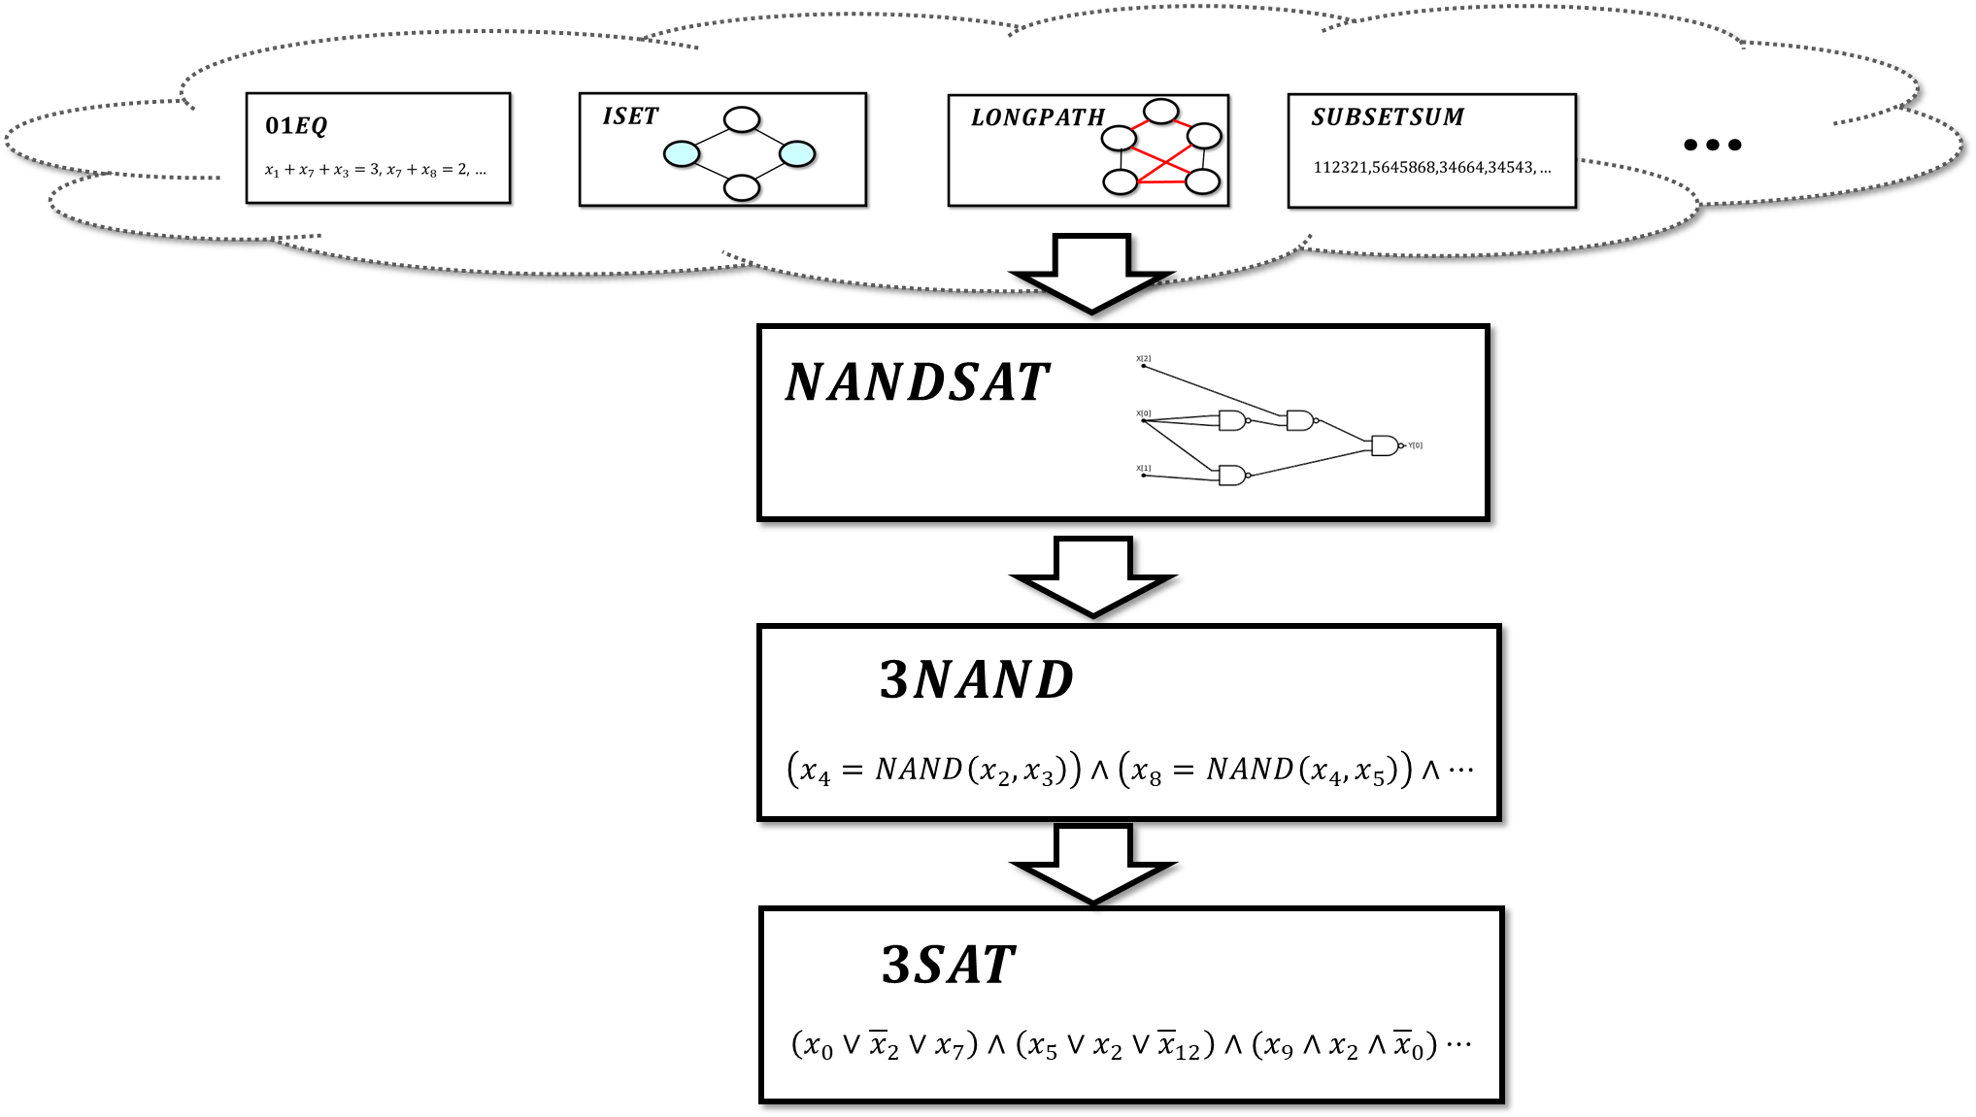
\includegraphics[width=\textwidth, height=0.25\paperheight, keepaspectratio]{../figure/cooklevin_overview.png}
\caption{Overview of the results of this chapter. We define
\(\mathbf{NP}\) to contain all decision problems for which a solution
can be efficiently \emph{verified}. The main result of this chapter is
the \emph{Cook Levin Theorem} (\cref{cook-levin-thm}) which states that
\(3\ensuremath{\mathit{SAT}}\) has a polynomial-time algorithm if and
only if \emph{every} problem in \(\mathbf{NP}\) has a polynomial-time
algorithm. Another way to state this theorem is that
\(3\ensuremath{\mathit{SAT}}\) is \emph{\(\mathbf{NP}\) complete}. We
will prove the Cook-Levin theorem by defining the two intermediate
problems \(\ensuremath{\mathit{NANDSAT}}\) and
\(3\ensuremath{\mathit{NAND}}\), proving that
\(\ensuremath{\mathit{NANDSAT}}\) is \(\mathbf{NP}\) complete, and then
proving that
\(\ensuremath{\mathit{NANDSAT}} \leq_p 3\ensuremath{\mathit{NAND}} \leq_p 3\ensuremath{\mathit{SAT}}\).}
\label{cooklevin_overviewfig}
\end{figure}

\section{The class \(\mathbf{NP}\)}\label{The-class-mathbfNP}

To make the above precise, we will make the following mathematical
definition. we define the class \(\mathbf{NP}\) to contain all Boolean
functions that correspond to a \emph{search problem} of the form above.
That is, a Boolean function \(F\) is in \(\mathbf{NP}\) if \(F\) has the
form that on input a string \(x\), \(F(x)=1\) if and only if there
exists a ``solution'' string \(w\) such that the pair \((x,w)\)
satisfies some polynomial-time checkable condition. Formally,
\(\mathbf{NP}\) is defined as follows:


\begin{marginfigure}
\centering
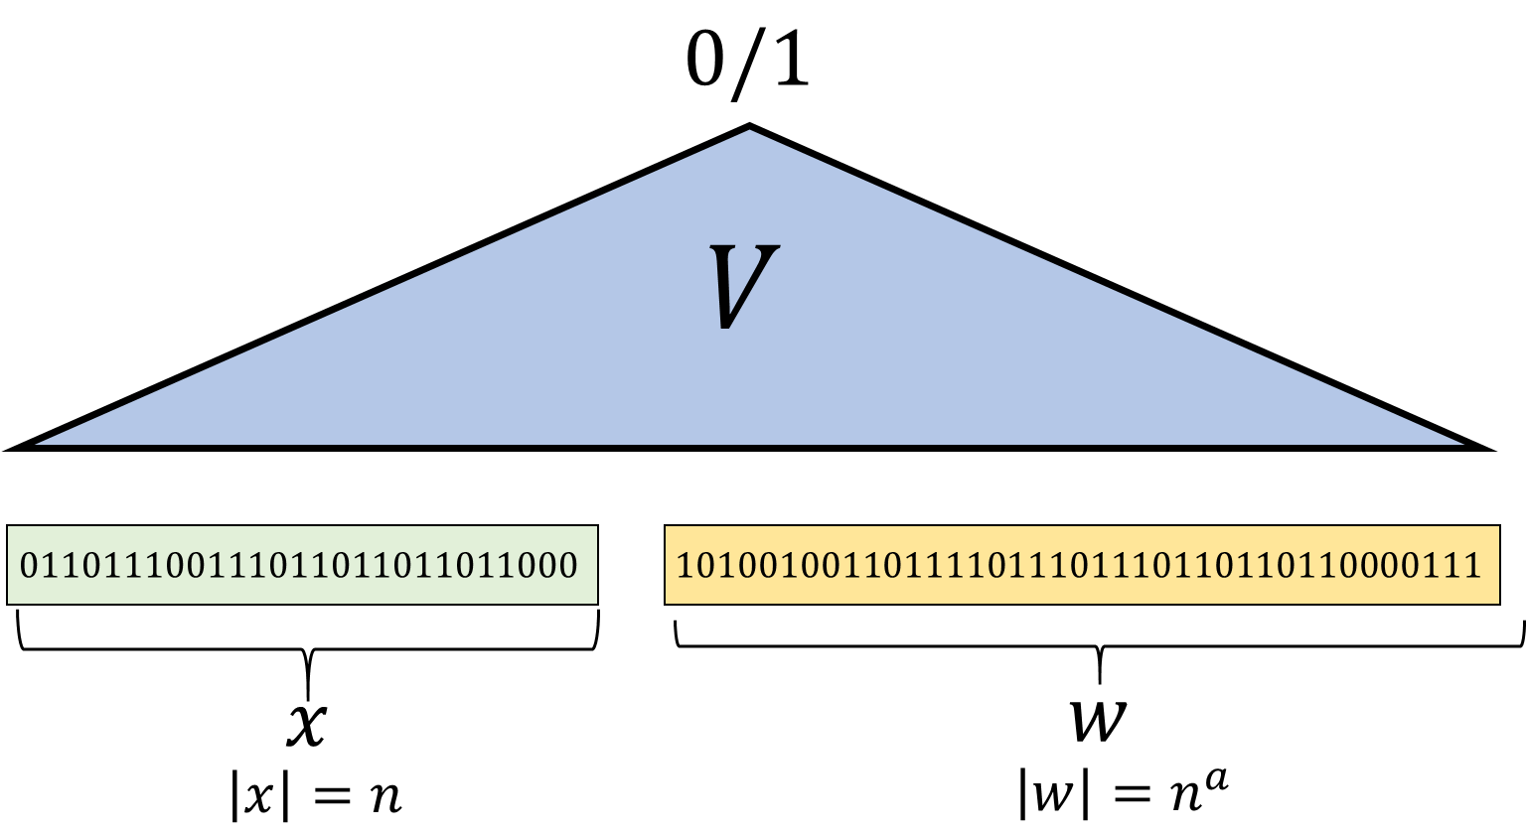
\includegraphics[width=\linewidth, height=1.5in, keepaspectratio]{../figure/NPdefinitionfig.png}
\caption{The class \(\mathbf{NP}\) corresponds to problems where
solutions can be \emph{efficiently verified}. That is, this is the class
of functions \(F\) such that \(F(x)=1\) if there is a ``solution'' \(w\)
of length polynomial in \(|x|\) that can be verified by a
polynomial-time algorithm \(V\).}
\label{NPdeffigfig}
\end{marginfigure}

\hypertarget{NP-def}{}
\begin{definition}[NP] \label[definition]{NP-def}

We say that \(F:\{0,1\}^* \rightarrow \{0,1\}\) is in \(\mathbf{NP}\) if
there exists some integer \(a>0\) and
\(V:\{0,1\}^* \rightarrow \{0,1\}\) such that \(V\in \mathbf{P}\) and
for every \(x\in \{0,1\}^n\), \[
F(x)=1 \Leftrightarrow \exists_{w \in \{0,1\}^{n^a}} \text{ s.t. } V(xw)=1 \;. \label{NP-eq}
\]

\end{definition}

In other words, for \(F\) to be in \(\mathbf{NP}\), there needs to exist
some polynomial-time computable verification function \(V\), such that
if \(F(x)=1\) then there must exist \(w\) (of length polynomial in
\(|x|\)) such that \(V(xw)=1\), and if \(F(x)=0\) then for \emph{every}
such \(w\), \(V(xw)=0\). Since the existence of this string \(w\)
certifies that \(F(x)=1\), \(w\) is often referred to as a
\emph{certificate}, \emph{witness}, or \emph{proof} that \(F(x)=1\).

See also \cref{NPdeffigfig} for an illustration of \cref{NP-def}. The
name \(\mathbf{NP}\) stands for ``nondeterministic polynomial time'' and
is used for historical reasons; see the bibiographical notes. The string
\(w\) in \eqref{NP-eq} is sometimes known as a \emph{solution},
\emph{certificate}, or \emph{witness} for the instance \(x\).

\hypertarget{NPalternativeex}{}
\begin{solvedexercise}[Alternative definition of $\mathbf{NP}$] \label[solvedexercise]{NPalternativeex}

Show that the condition that \(|w|=|x|^a\) in \cref{NP-def} can be
replaced by the condition that \(|w| \leq p(|x|)\) for some polynomial
\(p\). That is, prove that for every
\(F:\{0,1\}^* \rightarrow \{0,1\}\), \(F \in \mathbf{NP}\) if and only
if there is a polynomial-time Turing machine \(V\) and a polynomial
\(p:\N \rightarrow \N\) such that for every \(x\in \{0,1\}^*\)
\(F(x)=1\) if and only if there exists \(w\in \{0,1\}^*\) with
\(|w| \leq p(|x|)\) such that \(V(x,w)=1\).

\end{solvedexercise}

\begin{solution} \label[solution]{The-only-if-direction-nam}

The ``only if'' direction (namely that if \(F\in \mathbf{NP}\) then
there is an algorithm \(V\) and a polynomial \(p\) as above) follows
immediately from \cref{NP-def} by letting \(p(n)=n^a\). For the ``if''
direction, the idea is that if a string \(w\) is of size at most
\(p(n)\) for degree \(d\) polynomial \(p\), then there is some \(n_0\)
such that for all \(n > n_0\), \(|w| < n^{d+1}\). Hence we can encode
\(w\) by a string of exactly length \(n^{d+1}\) by padding it with \(1\)
and an appropriate number of zeroes. Hence if there is an algorithm
\(V\) and polynomial \(p\) as above, then we can define an algorithm
\(V'\) that does the following on input \(x,w'\) with \(|x|=n\) and
\(|w'|=n^a\):

\begin{itemize}
\item
  If \(n \leq n_0\) then \(V'(x,w')\) ignores \(w'\) and enumerates over
  all \(w\) of length at most \(p(n)\) and outputs \(1\) if there exists
  \(w\) such that \(V(x,w)=1\). (Since \(n < n_0\), this only takes a
  constant number of steps.)
\item
  If \(n> n_0\) then \(V'(x,w')\) ``strips out'' the padding by dropping
  all the rightmost zeroes from \(w\) until it reaches out the first
  \(1\) (which it drops as well) and obtains a string \(w\). If
  \(|w| \leq p(n)\) tnen \(V'\) outputs \(V(x,w)\).
\end{itemize}

Since \(V\) runs in polynomial time, \(V'\) runs in polynomial time as
well, and by definition for every \(x\), there exists
\(w' \in \{0,1\}^{|x|^a}\) such that \(V'(xw')=1\) if and only if there
exists \(w \in \{0,1\}^*\) with \(|w| \leq p(|x|)\) such that
\(V(xw)=1\).

\end{solution}

The definition of \(\mathbf{NP}\) means that for every
\(F\in \mathbf{NP}\) and string \(x\in \{0,1\}^*\), \(F(x)=1\) if and
only if there is a \emph{short and efficiently verifiable proof} of this
fact. That is, we can think of the function \(V\) in \cref{NP-def} as a
\emph{verifier} algorithm, similar to what we've seen in
\cref{godelproofdef}. The verifier checks whether a given string
\(w\in \{0,1\}^*\) is a valid proof for the statement ``\(F(x)=1\)''.
Essentially all proof systems considered in mathematics involve
line-by-line checks that can be carried out in polynomial time. Thus the
heart of \(\mathbf{NP}\) is asking for statements that have \emph{short}
(i.e., polynomial in the size of the statements) proof. Indeed, as we
will see in \cref{chappvsnp}, Kurt Gödel phrased the question of whether
\(\mathbf{NP}=\mathbf{P}\) as asking whether ``the mental work of a
mathematician {[}in proving theorems{]} could be completely replaced by
a machine''.

\hypertarget{NPassymetric}{}
\begin{remark}[$\mathbf{NP}$ not (necessaily) closed under complement] \label[remark]{NPassymetric}

\cref{NP-def} is \emph{asymmetric} in the sense that there is a
difference between an output of \(1\) and an output of \(0\). You should
make sure you understand why this definition does \emph{not} guarantee
that if \(F \in \mathbf{NP}\) then the function \(1-F\) (i.e., the map
\(x \mapsto 1-F(x)\)) is in \(\mathbf{NP}\) as well.

In fact, it is believed that there do exist functions \(F\) such that
\(F\in \mathbf{NP}\) but \(1-F \not\in \mathbf{NP}\). For example, as
shown below, \(3\ensuremath{\mathit{SAT}} \in \mathbf{NP}\), but the
function \(\overline{3\ensuremath{\mathit{SAT}}}\) that on input a 3CNF
formula \(\varphi\) outputs \(1\) if and only if \(\varphi\) is
\emph{not} satisfiable is not known (nor believed) to be in
\(\mathbf{NP}\). This is in contrast to the class \(\mathbf{P}\) which
\emph{does} satisfy that if \(F\in \mathbf{P}\) then \(1-F\) is in
\(\mathbf{P}\) as well.

\end{remark}

\subsection{Examples of functions in
\(\mathbf{NP}\)}\label{Examples-of-functions-in-}

We now present some examples of functions that are in the class
\(\mathbf{NP}\). We start with the canonical example of the
\(3\ensuremath{\mathit{SAT}}\) function.

\hypertarget{threesatinnpex}{}
\begin{example}[$3SAT \in \mathbf{NP}$] \label[example]{threesatinnpex}

\(3\ensuremath{\mathit{SAT}}\) is in \(\mathbf{NP}\) since for every
\(\ell\)-variable formula \(\varphi\),
\(3\ensuremath{\mathit{SAT}}(\varphi)=1\) if and only if there exists a
satisfying assignment \(x \in \{0,1\}^\ell\) such that \(\varphi(x)=1\),
and we can check this condition in polynomial time.

The above reasoning explains why \(3\ensuremath{\mathit{SAT}}\) is in
\(\mathbf{NP}\), but since this is our first example, we will now
belabor the point and expand out in full formality the precise
representation of the witness \(w\) and the algorithm \(V\) that
demonstrate that \(3\ensuremath{\mathit{SAT}}\) is in \(\mathbf{NP}\).
Since demonstrating that functions are in \(\mathbf{NP}\) is fairly
straightforward, in future cases we will not use as much detail, and the
reader can also feel free to skip the rest of this example.

Using \cref{NPalternativeex}, it is OK if witness is of size at most
polynomial in the input length \(n\), rather than of precisely size
\(n^a\) for some integer \(a>0\). Specifically, we can represent a 3CNF
formula \(\varphi\) with \(k\) variables and \(m\) clauses as a string
of length \(n=O(m\log k)\), since every one of the \(m\) clauses
involves three variables and their negation, and the identity of each
variable can be represented using \(\lceil \log_2 k \rceil\). We assume
that every variable participates in some clause (as otherwise it can be
ignored) and hence that \(m \geq k\), which in particular means that the
input length \(n\) is at least as large as \(m\) and \(k\).

We can represent an assignment to the \(k\) variables using a
\(k\)-length string \(w\). The following algorithm checks whether a
given \(w\) satisfies the formula \(\varphi\):

\begin{algorithm}[Verifier for $3SAT$]
\label[algorithm]{threesatverifieralg} ~ \\ \noindent
\begin{algorithmic}[1]
\INPUT  3CNF formula $\varphi$ on $k$ variables and with $m$ clauses, string $w \in \{0,1\}^k$ 
\OUTPUT  $1$ iff $w$ satisfies $\varphi$ 
\FOR{$j \in [m]$}
   \STATE Let $\ell_1 \vee \ell_2 \vee \ell_j$ be the $j$-th clause of $\varphi$ 
   \IF{$w$ violates all three literals}
     \RETURN $0$
   \ENDIF
\ENDFOR
\RETURN $1$
\end{algorithmic}
\end{algorithm}

\cref{threesatverifieralg} takes \(O(m)\) time to enumerate over all
clauses, and will return \(1\) if and only if \(y\) satisfies all the
clauses.

\end{example}

Here are some more examples for problems in \(\mathbf{NP}\). For each
one of these problems we merely sketch how the witness is represented
and why it is efficiently checkable, but working out the details can be
a good way to get more comfortable with \cref{NP-def}:

\begin{itemize}
\item
  \(\ensuremath{\mathit{QUADEQ}}\) is in \(\mathbf{NP}\) since for every
  \(\ell\)-variable instance of quadratic equations \(E\),
  \(\ensuremath{\mathit{QUADEQ}}(E)=1\) if and only if there exists an
  assignment \(x\in \{0,1\}^\ell\) that satisfies \(E\). We can check
  the condition that \(x\) satisfies \(E\) in polynomial time by
  enumerating over all the equations in \(E\), and for each such
  equation \(e\), plug in the values of \(x\) and verify that \(e\) is
  satisfied.
\item
  \(\ensuremath{\mathit{ISET}}\) is in \(\mathbf{NP}\) since for every
  graph \(G\) and integer \(k\), \(\ensuremath{\mathit{ISET}}(G,k)=1\)
  if and only if there exists a set \(S\) of \(k\) vertices that
  contains no pair of neighbors in \(G\). We can check the condition
  that \(S\) is an independent set of size \(\geq k\) in polynomial time
  by first checking that \(|S| \geq k\) and then enumerating over all
  edges \(\{u,v \}\) in \(G\), and for each such edge verify that either
  \(u\not\in S\) or \(v\not\in S\).
\item
  \(\ensuremath{\mathit{LONGPATH}}\) is in \(\mathbf{NP}\) since for
  every graph \(G\) and integer \(k\),
  \(\ensuremath{\mathit{LONGPATH}}(G,k)=1\) if and only if there exists
  a simple path \(P\) in \(G\) that is of length at least \(k\). We can
  check the condition that \(P\) is a simple path of length \(k\) in
  polynomial time by checking that it has the form
  \((v_0,v_1,\ldots,v_k)\) where each \(v_i\) is a vertex in \(G\), no
  \(v_i\) is repeated, and for every \(i \in [k]\), the edge
  \(\{v_i,v_{i+1}\}\) is present in the graph.
\item
  \(\ensuremath{\mathit{MAXCUT}}\) is in \(\mathbf{NP}\) since for every
  graph \(G\) and integer \(k\), \(\ensuremath{\mathit{MAXCUT}}(G,k)=1\)
  if and only if there exists a cut \((S,\overline{S})\) in \(G\) that
  cuts at least \(k\) edges. We can check that condition that
  \((S,\overline{S})\) is a cut of value at least \(k\) in polynomial
  time by checking that \(S\) is a subset of \(G\)'s vertices and
  enumerating over all the edges \(\{u,v\}\) of \(G\), counting those
  edges such that \(u\in S\) and \(v\not\in S\) or vice versa.
\end{itemize}

\subsection{Basic facts about
\(\mathbf{NP}\)}\label{Basic-facts-about-mathbfN}

The definition of \(\mathbf{NP}\) is one of the most important
definitions of this book, and is worth while taking the time to digest
and internalize. The following solved exercises establish some basic
properties of this class. As usual, I highly recommend that you try to
work out the solutions yourself.

\hypertarget{PinNP}{}
\begin{solvedexercise}[Verifying is no harder than solving] \label[solvedexercise]{PinNP}

Prove that \(\mathbf{P} \subseteq \mathbf{NP}\).

\end{solvedexercise}

\begin{solution} \label[solution]{Suppose-that-F-in-mathbfP}

Suppose that \(F \in \mathbf{P}\). Define the following function \(V\):
\(V(x0^n)=1\) iff \(n=|x|\) and \(F(x)=1\). (\(V\) outputs \(0\) on all
other inputs.) Since \(F\in \mathbf{P}\) we can clearly compute \(V\) in
polynomial time as well.

Let \(x\in \{0,1\}^n\) be some string. If \(F(x)=1\) then \(V(x0^n)=1\).
On the other hand, if \(F(x)=0\) then for every \(w\in \{0,1\}^n\),
\(V(xw)=0\). Therefore, setting \(a=b=1\), we see that \(V\) satisfies
\eqref{NP-eq}, and establishes that \(F \in \mathbf{NP}\).

\end{solution}

\hypertarget{NPandNOTPolynomial}{}
\begin{remark}[$\mathbf{NP}$ does not mean non-polynomial!] \label[remark]{NPandNOTPolynomial}

People sometimes think that \(\mathbf{NP}\) stands for ``non polynomial
time''. As \cref{PinNP} shows, this is far from the truth, and in fact
every polynomial-time computable function is in \(\mathbf{NP}\) as well.

If \(F\) is in \(\mathbf{NP}\) it certainly does \emph{not} mean that
\(F\) is hard to compute (though it does not, as far as we know,
necessarily mean that it's easy to compute either). Rather, it means
that \(F\) is \emph{easy to verify}, in the technical sense of
\cref{NP-def}.

\end{remark}

\hypertarget{NPinEXP}{}
\begin{solvedexercise}[$\mathbf{NP}$ is in exponential time] \label[solvedexercise]{NPinEXP}

Prove that \(\mathbf{NP} \subseteq \mathbf{EXP}\).

\end{solvedexercise}

\begin{solution} \label[solution]{Suppose-that-Fin-mathbfNP}

Suppose that \(F\in \mathbf{NP}\) and let \(V\) be the polynomial-time
computable function that satisfies \eqref{NP-eq} and \(a\) the
corresponding constant. Then given every \(x\in \{0,1\}^n\), we can
check whether \(F(x)=1\) in time
\(poly(n)\cdot 2^{n^a} = o(2^{n^{a+1}})\) by enumerating over all the
\(2^{n^a}\) strings \(w\in \{0,1\}^{n^a}\) and checking whether
\(V(xw)=1\), in which case we return \(1\). If \(V(xw)=0\) for every
such \(w\) then we return \(0\). By construction, the algorithm above
will run in time at most exponential in its input length and by the
definition of \(\mathbf{NP}\) it will return \(F(x)\) for every \(x\).

\end{solution}

\cref{PinNP} and \cref{NPinEXP} together imply that

\[\mathbf{P} \subseteq \mathbf{NP} \subseteq \mathbf{EXP}\;.\]

The time hierarchy theorem (\cref{time-hierarchy-thm}) implies that
\(\mathbf{P} \subsetneq \mathbf{EXP}\) and hence at least one of the two
inclusions \(\mathbf{P} \subseteq \mathbf{NP}\) or
\(\mathbf{NP} \subseteq \mathbf{EXP}\) is \emph{strict}. It is believed
that both of them are in fact strict inclusions. That is, it is believed
that there are functions in \(\mathbf{NP}\) that cannot be computed in
polynomial time (this is the \(\mathbf{P} \neq \mathbf{NP}\) conjecture)
and that there are functions \(F\) in \(\mathbf{EXP}\) for which we
cannot even efficiently \emph{certify} that \(F(x)=1\) for a given input
\(x\). One function \(F\) that is believed to lie in
\(\mathbf{EXP} \setminus \mathbf{NP}\) is the function
\(\overline{3\ensuremath{\mathit{SAT}}}\) defined as
\(\overline{3\ensuremath{\mathit{SAT}}}(\varphi)= 1 - 3\ensuremath{\mathit{SAT}}(\varphi)\)
for every 3CNF formula \(\varphi\). The conjecture that
\(\overline{3\ensuremath{\mathit{SAT}}}\not\in \mathbf{NP}\) is known as
the ``\(\mathbf{NP} \neq \mathbf{co-NP}\)'' conjecture. It implies the
\(\mathbf{P} \neq \mathbf{NP}\) conjecture (see \cref{npconppnpex}).

We have previously informally equated the notion of \(F \leq_p G\) with
\(F\) being ``no harder than \(G\)'' and in particular have seen in
\cref{reductionsandP} that if \(G \in \mathbf{P}\) and \(F \leq_p G\),
then \(F \in \mathbf{P}\) as well. The following exercise shows that if
\(F \leq_p G\) then it is also ``no harder to verify'' than \(G\). That
is, regardless of whether or not it is in \(\mathbf{P}\), if \(G\) has
the property that solutions to it can be efficiently verified, then so
does \(F\).

\hypertarget{reductionnpex}{}
\begin{solvedexercise}[Reductions and $\mathbf{NP}$] \label[solvedexercise]{reductionnpex}

Let \(F,G:\{0,1\}^* \rightarrow \{0,1\}\). Show that if \(F \leq_p G\)
and \(G\in \mathbf{NP}\) then \(F \in \mathbf{NP}\).

\end{solvedexercise}

\begin{solution} \label[solution]{Suppose-that-G-is-in-math}

Suppose that \(G\) is in \(\mathbf{NP}\) and in particular there exists
\(a\) and \(V \in \mathbf{P}\) such that for every \(y \in \{0,1\}^*\),
\(G(y)=1 \Leftrightarrow \exists_{w\in \{0,1\}^{|y|^a}} V(yw)=1\).
Suppose also that \(F \leq_p G\) and so in particular there is a
\(n^b\)-time computable function \(R\) such that \(F(x) = G(R(x))\) for
all \(x\in \{0,1\}^*\). Define \(V'\) to be a Turing Machine that on
input a pair \((x,w)\) computes \(y=R(x)\) and returns \(1\) if and only
if \(|w|=|y|^a\) and \(V(yw)=1\). Then \(V'\) runs in polynomial time,
and for every \(x\in \{0,1\}^*\), \(F(x)=1\) iff there exists \(w\) of
size \(|R(x)|^a\) which is at most polynomial in \(|x|\) such that
\(V'(x,w)=1\), hence demonstrating that \(F \in \mathbf{NP}\).

\end{solution}

\section{From \(\mathbf{NP}\) to 3SAT: The Cook-Levin
Theorem}\label{From-mathbfNP-to-SAT-The-}

We have seen everal example of problems for which we do not know if
their best algorithm is polynomial or exponential, but we can show that
they are in \(\mathbf{NP}\). That is, we don't know if they are easy to
\emph{solve}, but we do know that it is easy to \emph{verify} a given
solution. There are many, many, \emph{many}, more examples of
interesting functions we would like to compute that are easily shown to
be in \(\mathbf{NP}\). What is quite amazing is that if we can solve
3SAT then we can solve all of them!

The following is one of the most fundamental theorems in Computer
Science:

\hypertarget{cook-levin-thm}{}
\begin{theorem}[Cook-Levin Theorem] \label[theorem]{cook-levin-thm}

For every \(F\in \mathbf{NP}\), \(F \leq_p 3\ensuremath{\mathit{SAT}}\).

\end{theorem}

We will soon show the proof of \cref{cook-levin-thm}, but note that it
immediately implies that \(\ensuremath{\mathit{QUADEQ}}\),
\(\ensuremath{\mathit{LONGPATH}}\), and \(\ensuremath{\mathit{MAXCUT}}\)
all reduce to \(3\ensuremath{\mathit{SAT}}\). Combining it with the
reductions we've seen in \cref{reductionchap}, it implies that all these
problems are \emph{equivalent!} For example, to reduce
\(\ensuremath{\mathit{QUADEQ}}\) to \(\ensuremath{\mathit{LONGPATH}}\),
we can first reduce \(\ensuremath{\mathit{QUADEQ}}\) to
\(3\ensuremath{\mathit{SAT}}\) using \cref{cook-levin-thm} and use the
reduction we've seen in \cref{longpaththm} from
\(3\ensuremath{\mathit{SAT}}\) to \(\ensuremath{\mathit{LONGPATH}}\).
That is, since \(\ensuremath{\mathit{QUADEQ}} \in \mathbf{NP}\),
\cref{cook-levin-thm} implies that
\(\ensuremath{\mathit{QUADEQ}} \leq_p 3\ensuremath{\mathit{SAT}}\), and
\cref{longpaththm} implies that
\(3\ensuremath{\mathit{SAT}} \leq_p \ensuremath{\mathit{LONGPATH}}\),
which by the transitivity of reductions (\cref{transitiveex}) means that
\(\ensuremath{\mathit{QUADEQ}} \leq_p \ensuremath{\mathit{LONGPATH}}\).
Similarly, since \(\ensuremath{\mathit{LONGPATH}} \in \mathbf{NP}\), we
can use \cref{cook-levin-thm} and \cref{quadeq-thm} to show that
\(\ensuremath{\mathit{LONGPATH}} \leq_p 3\ensuremath{\mathit{SAT}} \leq_p \ensuremath{\mathit{QUADEQ}}\),
concluding that \(\ensuremath{\mathit{LONGPATH}}\) and
\(\ensuremath{\mathit{QUADEQ}}\) are computationally equivalent.

There is of course nothing special about
\(\ensuremath{\mathit{QUADEQ}}\) and \(\ensuremath{\mathit{LONGPATH}}\)
here: by combining \eqref{cook-levin-thm} with the reductions we saw, we
see that just like \(3\ensuremath{\mathit{SAT}}\), \emph{every}
\(F\in \mathbf{NP}\) reduces to \(\ensuremath{\mathit{LONGPATH}}\), and
the same is true for \(\ensuremath{\mathit{QUADEQ}}\) and
\(\ensuremath{\mathit{MAXCUT}}\). All these problems are in some sense
``the hardest in \(\mathbf{NP}\)'' since an efficient algorithm for any
one of them would imply an efficient algorithm for \emph{all} the
problems in \(\mathbf{NP}\). This motivates the following definition:

\hypertarget{NPC-def}{}
\begin{definition}[$\mathbf{NP}$-hardness and $\mathbf{NP}$-completeness] \label[definition]{NPC-def}

Let \(G:\{0,1\}^* \rightarrow \{0,1\}\). We say that \(G\) is
\emph{\(\mathbf{NP}\) hard} if for every \(F\in \mathbf{NP}\),
\(F \leq_p G\).

We say that \(G\) is \emph{\(\mathbf{NP}\) complete} if \(G\) is
\(\mathbf{NP}\) hard and \(G \in \mathbf{NP}\).

\end{definition}

The Cook-Levin Theorem (\cref{cook-levin-thm}) can be rephrased as
saying that \(3\ensuremath{\mathit{SAT}}\) is \(\mathbf{NP}\) hard, and
since it is also in \(\mathbf{NP}\), this means that
\(3\ensuremath{\mathit{SAT}}\) is \(\mathbf{NP}\) complete. Together
with the reductions of \cref{reductionchap}, \cref{cook-levin-thm} shows
that despite their superficial differences, 3SAT, quadratic equations,
longest path, independent set, and maximum cut, are all
\(\mathbf{NP}\)-complete. Many thousands of additional problems have
been shown to be \(\mathbf{NP}\)-complete, arising from all the
sciences, mathematics, economics, engineering and many other fields.
(For a few examples, see \href{https://goo.gl/NomnoU}{this Wikipedia
page} and \href{https://goo.gl/nfJHWv}{this website}.)

\hypertarget{npcomplete}{}
\begin{bigidea} \label[bigidea]{npcomplete}

If a \emph{single} \(\mathbf{NP}\)-complete has a polynomial-time
algorithm, then there is such an algorithm for every decision problem
that corresponds to the existence of an \emph{efficiently-verifiable}
solution.

\end{bigidea}

\subsection{What does this mean?}\label{What-does-this-mean}

As we've seen in \cref{PinNP}, \(\mathbf{P} \subseteq \mathbf{NP}\).
\emph{The} most famous conjecture in Computer Science is that this
containment is \emph{strict}. That is, it is widely conjectured that
\(\mathbf{P} \neq \mathbf{NP}\). One way to refute the conjecture that
\(\mathbf{P} \neq \mathbf{NP}\) is to give a polynomial-time algorithm
for even a single one of the \(\mathbf{NP}\)-complete problems such as
3SAT, Max Cut, or the thousands of others that have been studied in all
fields of human endeavors. The fact that these problems have been
studied by so many people, and yet not a single polynomial-time
algorithm for any of them has been found, supports that conjecture that
indeed \(\mathbf{P} \neq \mathbf{NP}\). In fact, for many of these
problems (including all the ones we mentioned above), we don't even know
of a \(2^{o(n)}\)-time algorithm! However, to the frustration of
computer scientists, we have not yet been able to prove that
\(\mathbf{P}\neq\mathbf{NP}\) or even rule out the existence of an
\(O(n)\)-time algorithm for 3SAT. Resolving whether or not
\(\mathbf{P}=\mathbf{NP}\) is known as the
\href{https://en.wikipedia.org/wiki/P_versus_NP_problem}{\(\mathbf{P}\)
vs \(\mathbf{NP}\) problem}. A million-dollar prize has been
\href{http://www.claymath.org/millennium-problems/p-vs-np-problem}{offered}
for the solution of this problem, a
\href{https://www.amazon.com/dp/B00BKZYGUY}{popular book} has been
written, and every year a new paper comes out claiming a proof of
\(\mathbf{P}=\mathbf{NP}\) or \(\mathbf{P}\neq\mathbf{NP}\), only to
wither under scrutiny.


\begin{marginfigure}
\centering
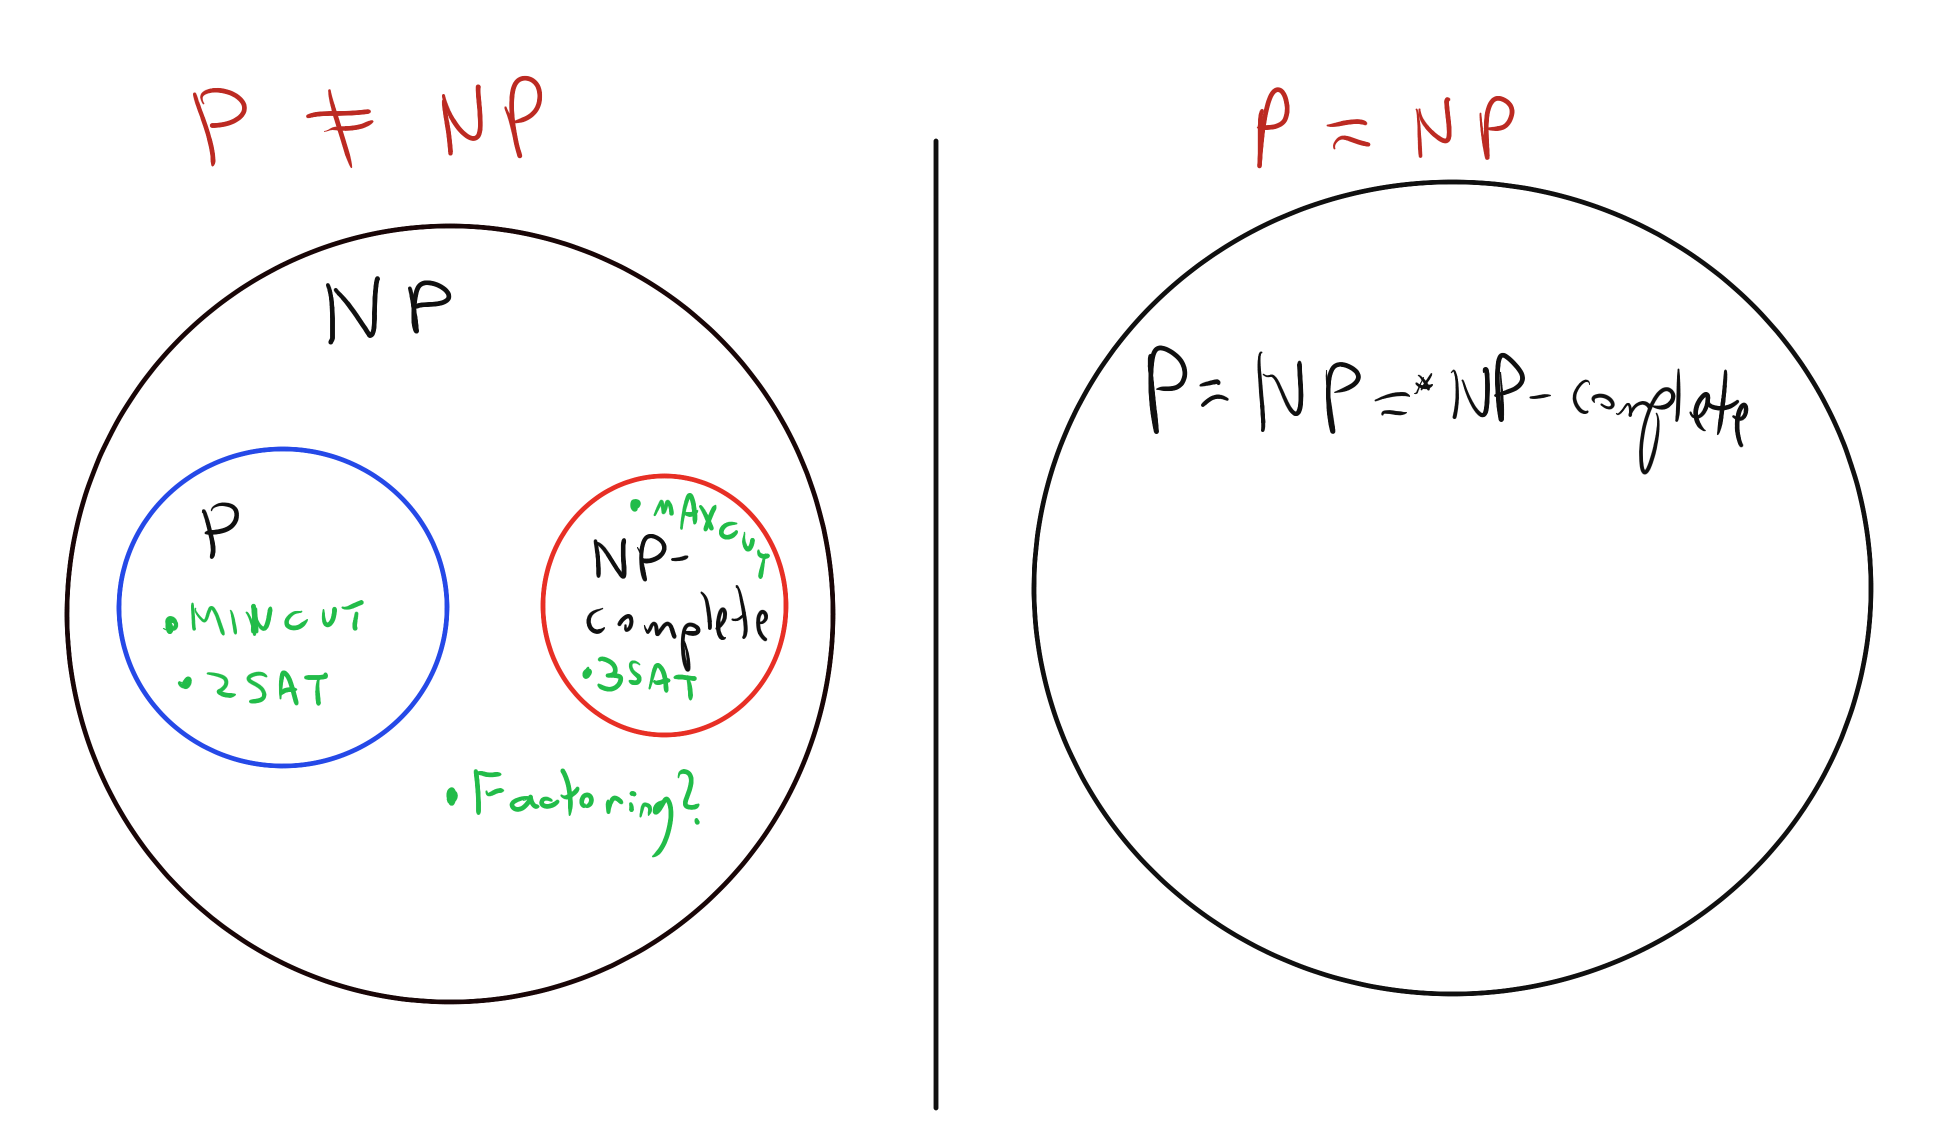
\includegraphics[width=\linewidth, height=1.5in, keepaspectratio]{../figure/PNPscenarios.png}
\caption{The world if \(\mathbf{P}\neq \mathbf{NP}\) (left) and
\(\mathbf{P}=\mathbf{NP}\) (right). In the former case the set of
\(\mathbf{NP}\)-complete problems is disjoint from \(\mathbf{P}\) and
Ladner's theorem shows that there exist problems that are neither in
\(\mathbf{P}\) nor are \(\mathbf{NP}\)-complete. (There are remarkably
few natural candidates for such problems, with some prominent examples
being decision variants of problems such as integer factoring, lattice
shortest vector, and finding Nash equilibria.) In the latter case that
\(\mathbf{P}=\mathbf{NP}\) the notion of \(\mathbf{NP}\)-completeness
loses its meaning, as essentially all functions in \(\mathbf{P}\) (save
for the trivial constant zero and constant one functions) are
\(\mathbf{NP}\)-complete.}
\label{PNPscenariosfig}
\end{marginfigure}

One of the mysteries of computation is that people have observed a
certain empirical ``zero-one law'' or ``dichotomy'' in the computational
complexity of natural problems, in the sense that many natural problems
are either in \(\mathbf{P}\) (often in
\(\ensuremath{\mathit{TIME}}(O(n))\) or
\(\ensuremath{\mathit{TIME}}(O(n^2))\)), or they are are \(\mathbf{NP}\)
hard. This is related to the fact that for most natural problems, the
best known algorithm is either exponential or polynomial, with not too
many examples where the best running time is some strange intermediate
complexity such as \(2^{2^{\sqrt{\log n}}}\). However, it is believed
that there exist problems in \(\mathbf{NP}\) that are neither in
\(\mathbf{P}\) nor are \(\mathbf{NP}\)-complete, and in fact a result
known as ``Ladner's Theorem'' shows that if
\(\mathbf{P} \neq \mathbf{NP}\) then this is indeed the case (see also
\cref{ladner-ex} and \cref{PNPscenariosfig}).


\begin{marginfigure}
\centering
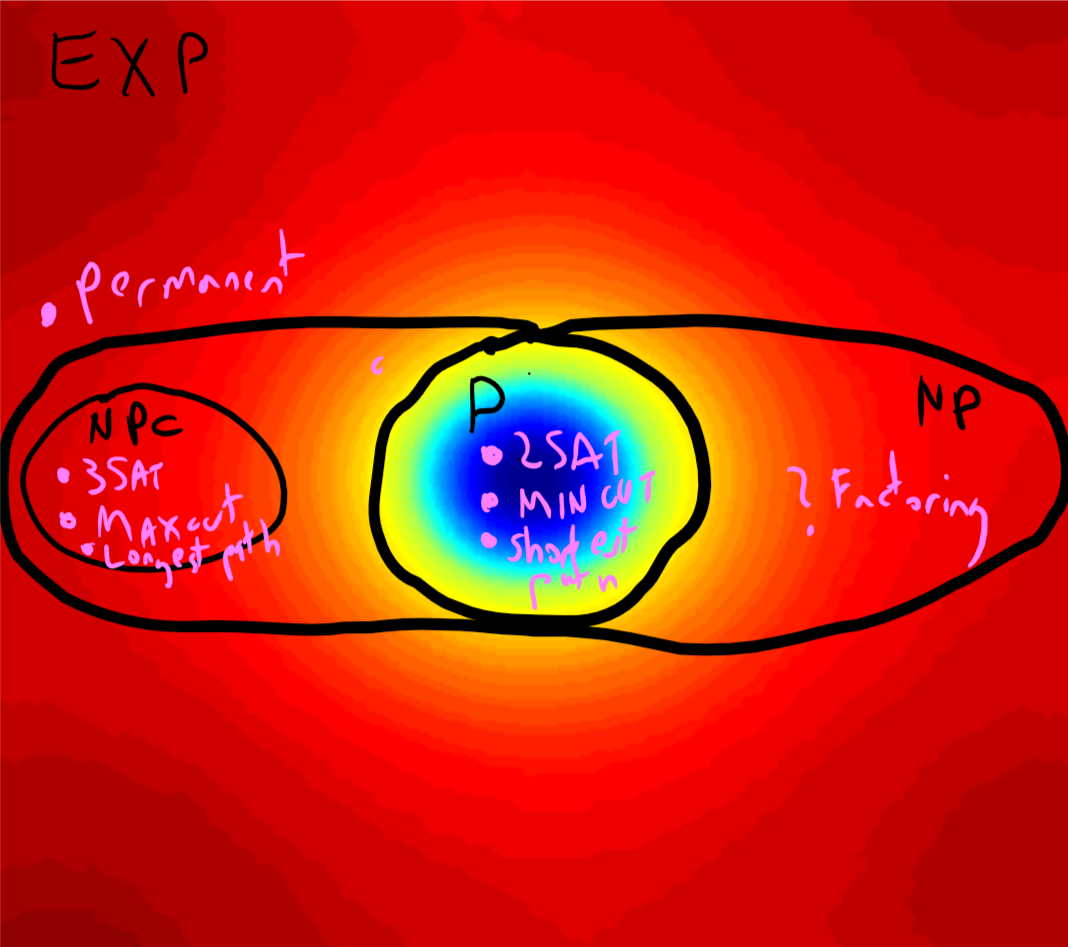
\includegraphics[width=\linewidth, height=1.5in, keepaspectratio]{../figure/PNPmap.png}
\caption{A rough illustration of the (conjectured) status of problems in
exponential time. Darker colors correspond to higher running time, and
the circle in the middle is the problems in \(\mathbf{P}\).
\(\mathbf{NP}\) is a (conjectured to be proper) superclass of
\(\mathbf{P}\) and the \(\mathbf{NP}\)-complete problems (or
\(\mathbf{NPC}\) for short) are the ``hardest'' problems in
\(\mathbf{NP}\), in the sense that a solution for one of them implies a
solution for all other problems in \(\mathbf{NP}\). It is conjectured
that all the \(\mathbf{NP}\)-complete problems require at least
\(\exp(n^\epsilon)\) time to solve for a constant \(\epsilon>0\), and
many require \(\exp(\Omega(n))\) time. The \emph{permanent} is not
believed to be contained in \(\mathbf{NP}\) though it is
\(\mathbf{NP}\)-hard, which means that a polynomial-time algorithm for
it implies that \(\mathbf{P}=\mathbf{NP}\).}
\label{complexitymapfig}
\end{marginfigure}

\subsection{The Cook-Levin Theorem: Proof
outline}\label{The-Cook-Levin-Theorem-Pr}

We will now prove the Cook-Levin Theorem, which is the underpinning to a
great web of reductions from 3SAT to thousands of problems across great
many fields. Some problems that have been shown to be
\(\mathbf{NP}\)-complete include: minimum-energy protein folding,
minimum surface-area foam configuration, map coloring, optimal Nash
equilibrium, quantum state entanglement, minimum supersequence of a
genome, minimum codeword problem, shortest vector in a lattice, minimum
genus knots, positive Diophantine equations, integer programming, and
many many more. The worst-case complexity of all these problems is (up
to polynomial factors) equivalent to that of 3SAT, and through the
Cook-Levin Theorem, to all problems in \(\mathbf{NP}\).

To prove \cref{cook-levin-thm} we need to show that
\(F \leq_p 3\ensuremath{\mathit{SAT}}\) for every \(F\in \mathbf{NP}\).
We will do so in three stages. We define two intermediate problems:
\(\ensuremath{\mathit{NANDSAT}}\) and \(3\ensuremath{\mathit{NAND}}\).
We will shortly show the definitions of these two problems, but
\cref{cook-levin-thm} will follow from combining the following three
results:

\begin{enumerate}
\def\labelenumi{\arabic{enumi}.}
\item
  \(\ensuremath{\mathit{NANDSAT}}\) is \(\mathbf{NP}\) hard
  (\cref{nand-thm}).
\item
  \(\ensuremath{\mathit{NANDSAT}} \leq_p 3\ensuremath{\mathit{NAND}}\)
  (\cref{threenand-thm}).
\item
  \(3\ensuremath{\mathit{NAND}} \leq_p 3\ensuremath{\mathit{SAT}}\)
  (\cref{threenand-sat-thm}).
\end{enumerate}

By the transitivity of reductions, it will follow that for every
\(F \in \mathbf{NP}\),

\[
F \leq_p \ensuremath{\mathit{NANDSAT}} \leq_p 3\ensuremath{\mathit{NAND}} \leq_p 3\ensuremath{\mathit{SAT}}
\]

hence establishing \cref{cook-levin-thm}.

We will prove these three results \cref{nand-thm}, \cref{threenand-thm}
and \cref{threenand-sat-thm} one by one, providing the requisite
definitions as we go along.

\section{The \(\ensuremath{\mathit{NANDSAT}}\) Problem, and why it is
\(\mathbf{NP}\) hard.}\label{The-ensuremathmathitNANDS}

The function
\(\ensuremath{\mathit{NANDSAT}}:\{0,1\}^* \rightarrow \{0,1\}\) is
defined as follows:

\begin{itemize}
\item
  The \textbf{input} to \(\ensuremath{\mathit{NANDSAT}}\) is a string
  \(Q\) representing a NAND-CIRC program (or equivalently, a circuit
  with NAND gates).
\item
  The \textbf{output} of \(\ensuremath{\mathit{NANDSAT}}\) on input
  \(Q\) is \(1\) if and only if there exists a string \(w\in \{0,1\}^n\)
  (where \(n\) is the number of inputs to \(Q\)) such that \(Q(w)=1\).
\end{itemize}

\hypertarget{NANDSATinNP}{}
\begin{solvedexercise}[$NANDSAT \in \mathbf{NP}$] \label[solvedexercise]{NANDSATinNP}

Prove that \(\ensuremath{\mathit{NANDSAT}} \in \mathbf{NP}\).

\end{solvedexercise}

\begin{solution} \label[solution]{We-have-seen-that-the-cir}

We have seen that the circuit (or straightline program) evaluation
problem can be computed in polynomial time. Specifically, given a
NAND-CIRC program \(Q\) of \(s\) lines and \(n\) inputs, and
\(w\in \{0,1\}^n\), we can evaluate \(Q\) on the input \(w\) in time
which is polynomial in \(s\) and hence verify whether or not \(Q(w)=1\).

\end{solution}

We now prove that \(\ensuremath{\mathit{NANDSAT}}\) is \(\mathbf{NP}\)
hard.

\hypertarget{nand-thm}{}
\begin{lemma} \label[lemma]{nand-thm}

\(\ensuremath{\mathit{NANDSAT}}\) is \(\mathbf{NP}\) hard.

\end{lemma}

\begin{proofidea} \label[proofidea]{The-proof-closely-follows}

The proof closely follows the proof that
\(\mathbf{P} \subseteq \mathbf{P_{/poly}}\) (\cref{non-uniform-thm} ,
see also \cref{unrollloopsec}). Specifically, if \(F\in \mathbf{NP}\)
then there is a polynomial time Turing machine \(M\) and positive
integer \(a\) such that for every \(x\in \{0,1\}^n\), \(F(x)=1\) iff
there is some \(w \in \{0,1\}^{n^a}\) such that \(M(xw)=1\). The proof
that \(\mathbf{P} \subseteq \mathbf{P_{/poly}}\) gave us way (via
``unrolling the loop'') to come up in polynomial time with a Boolean
circuit \(C\) on \(n^a\) inputs that computes the function
\(w \mapsto M(xw)\). We can then translate \(C\) into an equivalent NAND
circuit (or NAND-CIRC program) \(Q\). We see that there is a string
\(w \in \{0,1\}^{n^a}\) such that \(Q(w)=1\) if and only if there is
such \(w\) satisfying \(M(xw)=1\) which (by definition) happens if and
only if \(F(x)=1\). Hence the translation of \(x\) into the circuit
\(Q\) is a reduction showing \(F \leq_p \ensuremath{\mathit{NANDSAT}}\).

\end{proofidea}

\begin{pause} \label[pause]{The-proof-is-a-little-bit}

The proof is a little bit technical but ultimately follows quite
directly from the definition of \(\mathbf{NP}\), as well as the ability
to ``unroll the loop'' of NAND-TM programs as discussed in
\cref{unrollloopsec}. If you find it confusing, try to pause here and
think how you would implement in your favorite programming language the
function \texttt{unroll} which on input a NAND-TM program \(P\) and
numbers \(T,n\) outputs an \(n\)-input NAND-CIRC program \(Q\) of
\(O(|T|)\) lines such that for every input \(z\in \{0,1\}^n\), if \(P\)
halts on \(z\) within at most \(T\) steps and outputs \(y\), then
\(Q(z)=y\).

\end{pause}

\begin{proof}[Proof of \cref{nand-thm}] \label[proof]{Let-F-in-mathbfNP-To-prov}

Let \(F \in \mathbf{NP}\). To prove \cref{nand-thm} we need to give a
polynomial-time computable function that will map every
\(x^* \in \{0,1\}^*\) to a NAND-CIRC program \(Q\) such that
\(F(x)=\ensuremath{\mathit{NANDSAT}}(Q)\).

Let \(x^* \in \{0,1\}^*\) be such a string and let \(n=|x^*|\) be its
length. By \cref{NP-def} there exists \(V \in \mathbf{P}\) and positive
\(a \N\) such that \(F(x^*)=1\) if and only if there exists
\(w\in \{0,1\}^{n^a}\) satisfying \(V(x^*w)=1\).

Let \(m=n^a\). Since \(V\in \mathbf{P}\) there is some NAND-TM program
\(P^*\) that computes \(V\) on inputs of the form \(xw\) with
\(x\in \{0,1\}^n\) and \(w\in \{0,1\}^m\) in at most \({(n+m)}^c\) time
for some constant \(c\). Using our ``unrolling the loop NAND-TM to NAND
compiler'' of \cref{nand-compiler}, we can obtain a NAND-CIRC program
\(Q'\) that has \(n+m\) inputs and at most \(O((n+m)^{2c})\) lines such
that \(Q'(xw)= P^*(xw)\) for every \(x\in \{0,1\}^n\) and
\(w \in \{0,1\}^m\).

We can then use a simple ``hardwiring'' technique, reminiscent of
\cref{hardwiringrem} to map \(Q'\) into a circuit/NAND-CIRC program
\(Q\) on \(m\) inputs such that \(Q(w)= Q'(x^*w)\) for every
\(w\in \{0,1\}^m\).

\textbf{CLAIM:} There is a polynomial-time algorithm that on input a
NAND-CIRC program \(Q'\) on \(n+m\) inputs and \(x^* \in \{0,1\}^n\),
outputs a NAND-CIRC program \(Q\) such that for every
\(w\in \{0,1\}^n\), \(Q(w)=Q'(x^*w)\).

\textbf{PROOF OF CLAIM:} We can do so by adding a few lines to ensure
that the variables \texttt{zero} and \texttt{one} are \(0\) and \(1\)
respectively, and then simply replacing any reference in \(Q'\) to an
input \(x_i\) with \(i\in [n]\) the corresponding value based on
\(x^*_i\). See \cref{hardwiringfig} for an implementation of this
reduction in Python.

Our final reduction maps an input \(x^*\), into the NAND-CIRC program
\(Q\) obtained above. By the above discussion, this reduction runs in
polynomial time. Since we know that \(F(x^*)=1\) if and only if there
exists \(w\in \{0,1\}^m\) such that \(P^*(x^*w)=1\), this means that
\(F(x^*)=1\) if and only if \(\ensuremath{\mathit{NANDSAT}}(Q)=1\),
which is what we wanted to prove.

\end{proof}


\begin{figure}
\centering
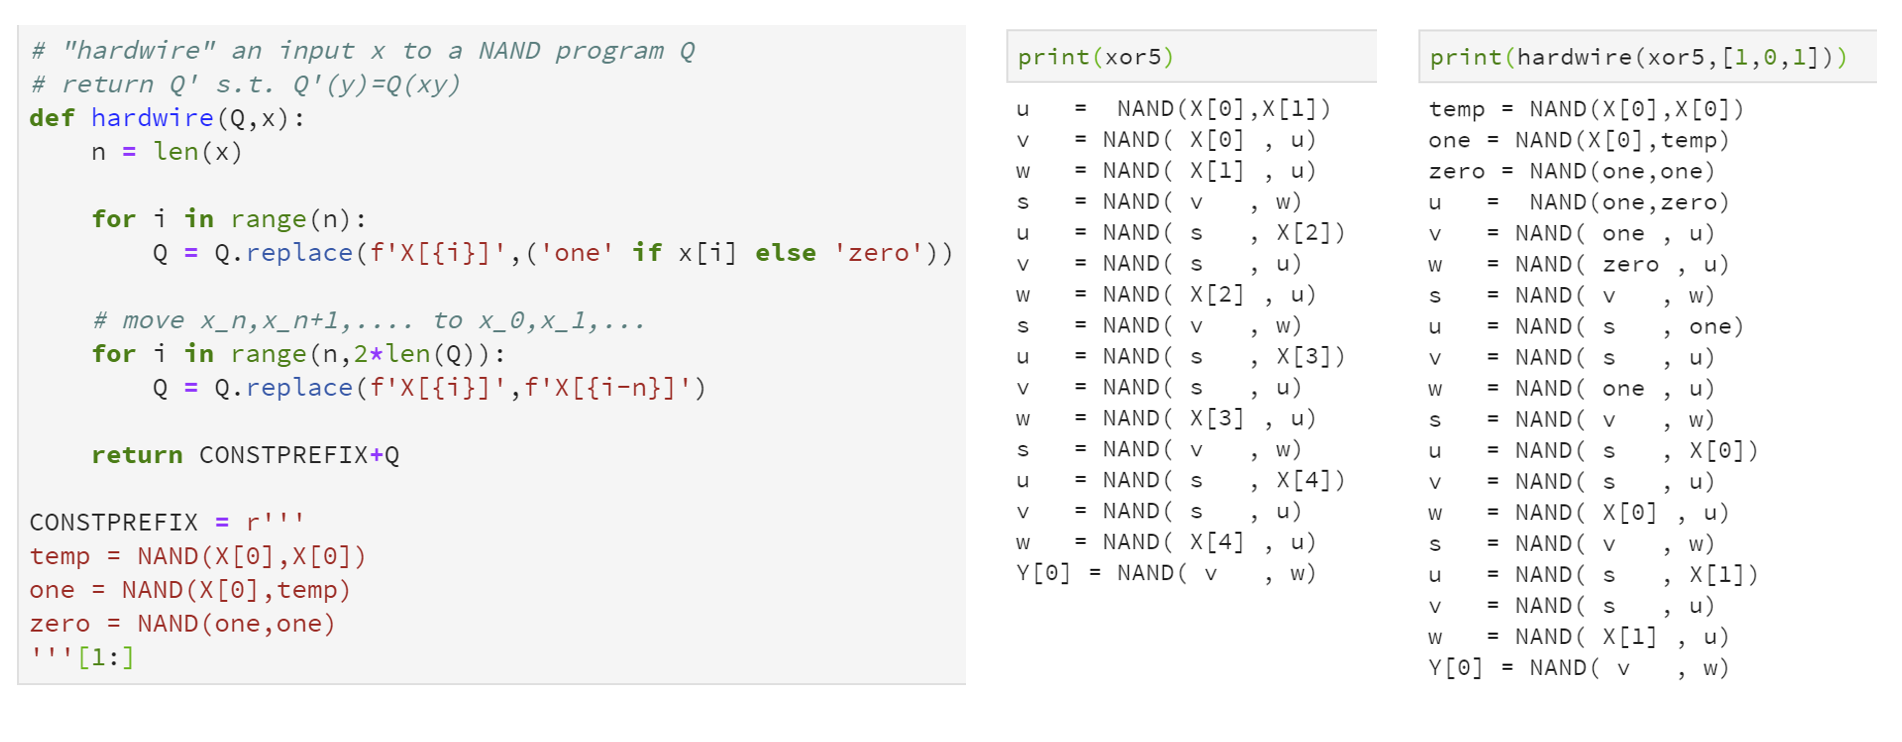
\includegraphics[width=\textwidth, height=0.25\paperheight, keepaspectratio]{../figure/hardwiring.png}
\caption{Given an \(T\)-line NAND-CIRC program \(Q\) that has \(n+m\)
inputs and some \(x^*\in \{0,1\}^n\), we can transform \(Q\) into a
\(T+3\) line NAND-CIRC program \(Q'\) that computes the map
\(w \mapsto Q(x^*w)\) for \(w\in \{0,1\}^m\) by simply adding code to
compute the \texttt{zero} and \texttt{one} constants, replacing all
references to \texttt{X[}\(i\)\texttt{]} with either \texttt{zero} or
\texttt{one} depending on the value of \(x^*_i\), and then replacing the
remaining references to \texttt{X[}\(j\)\texttt{]} with
\texttt{X[}\(j-n\)\texttt{]}. Above is Python code that implements this
transformation, as well as an example of its execution on a simple
program.}
\label{hardwiringfig}
\end{figure}

\section{The \(3\ensuremath{\mathit{NAND}}\)
problem}\label{The-ensuremathmathitNAND-}

The \(3\ensuremath{\mathit{NAND}}\) problem is defined as follows:

\begin{itemize}
\item
  The \textbf{input} is a logical formula \(\Psi\) on a set of variables
  \(z_0,\ldots,z_{r-1}\) which is an AND of constraints of the form
  \(z_i = \ensuremath{\mathit{NAND}}(z_j,z_k)\).
\item
  The \textbf{output} is \(1\) if and only if there is an input
  \(z\in \{0,1\}^r\) that satisfies all of the constraints.
\end{itemize}

For example, the following is a \(3\ensuremath{\mathit{NAND}}\) formula
with \(5\) variables and \(3\) constraints:

\[
\Psi = \left( z_3 = \ensuremath{\mathit{NAND}}(z_0,z_2) \right) \wedge \left( z_1 = \ensuremath{\mathit{NAND}}(z_0,z_2) \right) \wedge \left( z_4 = \ensuremath{\mathit{NAND}}(z_3,z_1) \right) \;.
\]

In this case \(3\ensuremath{\mathit{NAND}}(\Psi)=1\) since the
assignment \(z = 01010\) satisfies it. Given a
\(3\ensuremath{\mathit{NAND}}\) formula \(\Psi\) on \(r\) variables and
an assignment \(z\in \{0,1\}^r\), we can check in polynomial time
whether \(\Psi(z)=1\), and hence
\(3\ensuremath{\mathit{NAND}} \in \mathbf{NP}\). We now prove that
\(3\ensuremath{\mathit{NAND}}\) is \(\mathbf{NP}\) hard:

\hypertarget{threenand-thm}{}
\begin{lemma} \label[lemma]{threenand-thm}

\(\ensuremath{\mathit{NANDSAT}} \leq_p 3\ensuremath{\mathit{NAND}}\).

\end{lemma}

\begin{proofidea} \label[proofidea]{To-prove-crefthreenand-th}

To prove \cref{threenand-thm} we need to give a polynomial-time map from
every NAND-CIRC program \(Q\) to a 3NAND formula \(\Psi\) such that
there exists \(w\) such that \(Q(w)=1\) if and only if there exists
\(z\) satisfying \(\Psi\). For every line \(i\) of \(Q\), we define a
corresponding variable \(z_i\) of \(\Psi\). If the line \(i\) has the
form \texttt{foo = NAND(bar,blah)} then we will add the clause
\(z_i = \ensuremath{\mathit{NAND}}(z_j,z_k)\) where \(j\) and \(k\) are
the last lines in which \texttt{bar} and \texttt{blah} were written to.
We will also set variables corresponding to the input variables, as well
as add a clause to ensure that the final output is \(1\). The resulting
reduction can be implemented in about a dozen lines of Python, see
\cref{nandsattothreenandfig}.

\end{proofidea}


\begin{figure}
\centering
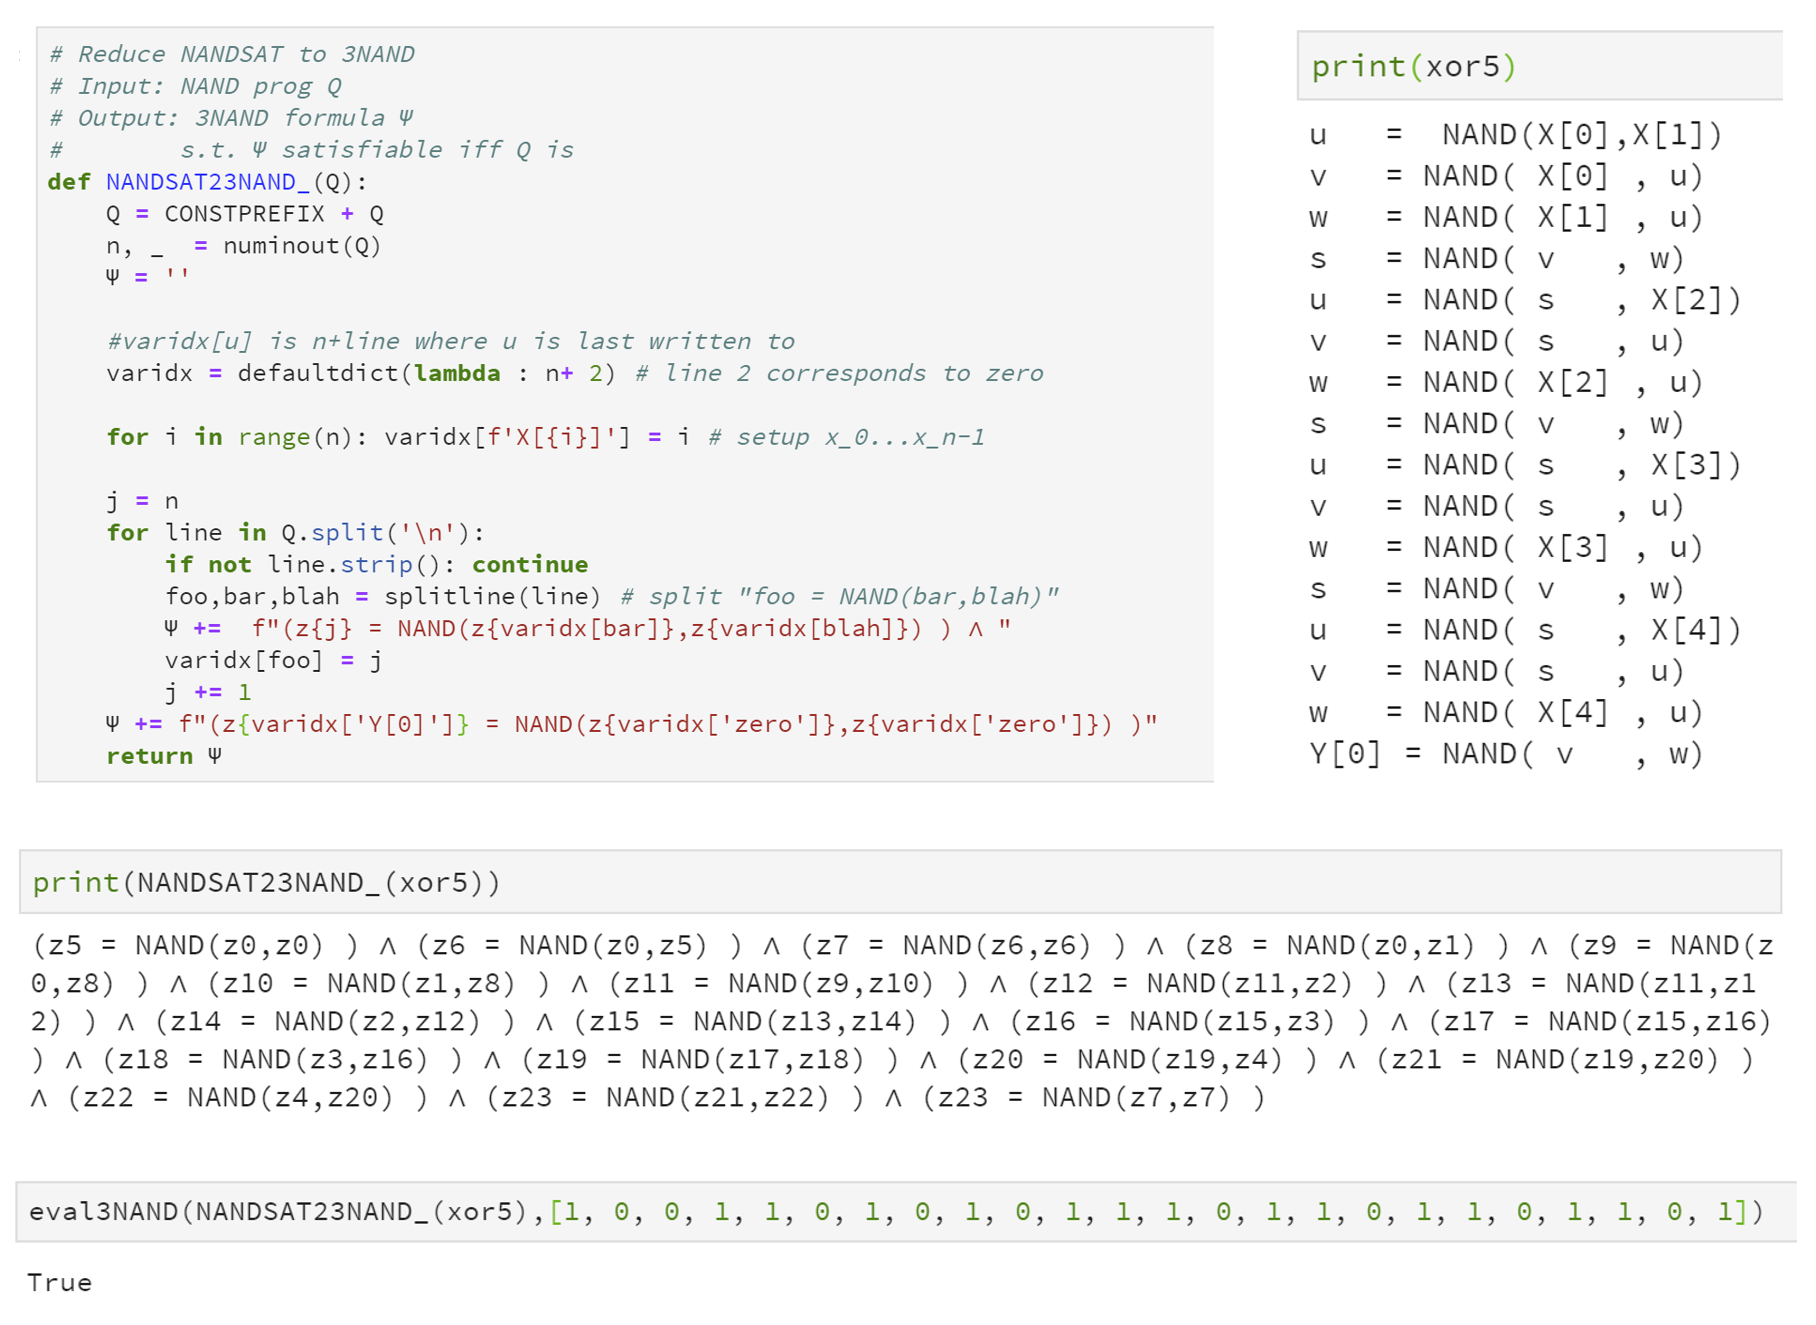
\includegraphics[width=\textwidth, height=0.25\paperheight, keepaspectratio]{../figure/nandsatto3nandreduction.png}
\caption{Python code to reduce an instance \(Q\) of
\(\ensuremath{\mathit{NANDSAT}}\) to an instance \(\Psi\) of
\(3\ensuremath{\mathit{NAND}}\). In the example above we transform the
NAND-CIRC program \texttt{xor5} which has \(5\) input variables and
\(16\) lines, into a \(3\ensuremath{\mathit{NAND}}\) formula \(\Psi\)
that has \(24\) variables and \(20\) clauses. Since \texttt{xor5}
outputs \(1\) on the input \(1,0,0,1,1\), there exists an assignment
\(z \in \{0,1\}^{24}\) to \(\Psi\) such that
\((z_0,z_1,z_2,z_3,z_4)=(1,0,0,1,1)\) and \(\Psi\) evaluates to
\emph{true} on \(z\).}
\label{nandsattothreenandfig}
\end{figure}

\begin{proof}[Proof of \cref{threenand-thm}] \label[proof]{To-prove-crefthreenand-th}

To prove \cref{threenand-thm} we need to give a reduction from
\(\ensuremath{\mathit{NANDSAT}}\) to \(3\ensuremath{\mathit{NAND}}\).
Let \(Q\) be a NAND-CIRC program with \(n\) inputs, one output, and
\(m\) lines. We can assume without loss of generality that \(Q\)
contains the variables \texttt{one} and \texttt{zero} as usual.

We map \(Q\) to a \(3\ensuremath{\mathit{NAND}}\) formula \(\Psi\) as
follows:

\begin{itemize}
\item
  \(\Psi\) has \(m+n\) variables \(z_0,\ldots,z_{m+n-1}\).
\item
  The first \(n\) variables \(z_0,\ldots,z_{n-1}\) will corresponds to
  the inputs of \(Q\). The next \(m\) variables \(z_n,\ldots,z_{n+m-1}\)
  will correspond to the \(m\) lines of \(Q\).
\item
  For every \(\ell\in \{n,n+1,\ldots,n+m \}\), if the \(\ell-n\)-th line
  of the program \(Q\) is \texttt{foo = NAND(bar,blah)} then we add to
  \(\Psi\) the constraint
  \(z_\ell = \ensuremath{\mathit{NAND}}(z_j,z_k)\) where \(j-n\) and
  \(k-n\) correspond to the last lines in which the variables
  \texttt{bar} and \texttt{blah} (respectively) were written to. If one
  or both of \texttt{bar} and \texttt{blah} was not written to before
  then we use \(z_{\ell_0}\) instead of the corresponding value \(z_j\)
  or \(z_k\) in the constraint, where \(\ell_0-n\) is the line in which
  \texttt{zero} is assigned a value. If one or both of \texttt{bar} and
  \texttt{blah} is an input variable \texttt{X[i]} then we use \(z_i\)
  in the constraint.
\item
  Let \(\ell^*\) be the last line in which the output \texttt{y\_0} is
  assigned a value. Then we add the constraint
  \(z_{\ell^*} = \ensuremath{\mathit{NAND}}(z_{\ell_0},z_{\ell_0})\)
  where \(\ell_0-n\) is as above the last line in which \texttt{zero} is
  assigned a value. Note that this is effectively the constraint
  \(z_{\ell^*}=\ensuremath{\mathit{NAND}}(0,0)=1\).
\end{itemize}

To complete the proof we need to show that there exists
\(w\in \{0,1\}^n\) s.t. \(Q(w)=1\) if and only if there exists
\(z\in \{0,1\}^{n+m}\) that satisfies all constraints in \(\Psi\). We
now show both sides of this equivalence.

\textbf{Part I: Completeness.} Suppose that there is \(w\in \{0,1\}^n\)
s.t. \(Q(w)=1\). Let \(z\in \{0,1\}^{n+m}\) be defined as follows: for
\(i\in [n]\), \(z_i=w_i\) and for \(i\in \{n,n+1,\ldots,n+m\}\) \(z_i\)
equals the value that is assigned in the \((i-n)\)-th line of \(Q\) when
executed on \(w\). Then by construction \(z\) satisfies all of the
constraints of \(\Psi\) (including the constraint that
\(z_{\ell^*}=\ensuremath{\mathit{NAND}}(0,0)=1\) since \(Q(w)=1\).)

\textbf{Part II: Soundness.} Suppose that there exists
\(z\in \{0,1\}^{n+m}\) satisfying \(\Psi\). Soundness will follow by
showing that \(Q(z_0,\ldots,z_{n-1})=1\) (and hence in particular there
exists \(w\in \{0,1\}^n\), namely \(w=z_0\cdots z_{n-1}\), such that
\(Q(w)=1\)). To do this we will prove the following claim \((*)\): for
every \(\ell \in [m]\), \(z_{\ell+n}\) equals the value assigned in the
\(\ell\)-th step of the execution of the program \(Q\) on
\(z_0,\ldots,z_{n-1}\). Note that because \(z\) satisfies the
constraints of \(\Psi\), \((*)\) is sufficient to prove the soundness
condition since these constraints imply that the last value assigned to
the variable \texttt{y\_0} in the execution of \(Q\) on
\(z_0\cdots w_{n-1}\) is equal to \(1\). To prove \((*)\) suppose,
towards a contradiction, that it is false, and let \(\ell\) be the
smallest number such that \(z_{\ell+n}\) is \emph{not} equal to the
value assigned in the \(\ell\)-th step of the execution of \(Q\) on
\(z_0,\ldots,z_{n-1}\). But since \(z\) satisfies the constraints of
\(\Psi\), we get that \(z_{\ell+n}=\ensuremath{\mathit{NAND}}(z_i,z_j)\)
where (by the assumption above that \(\ell\) is \emph{smallest} with
this property) these values \emph{do} correspond to the values last
assigned to the variables on the righthand side of the assignment
operator in the \(\ell\)-th line of the program. But this means that the
value assigned in the \(\ell\)-th step is indeed simply the NAND of
\(z_i\) and \(z_j\), contradicting our assumption on the choice of
\(\ell\).

\end{proof}


\begin{marginfigure}
\centering
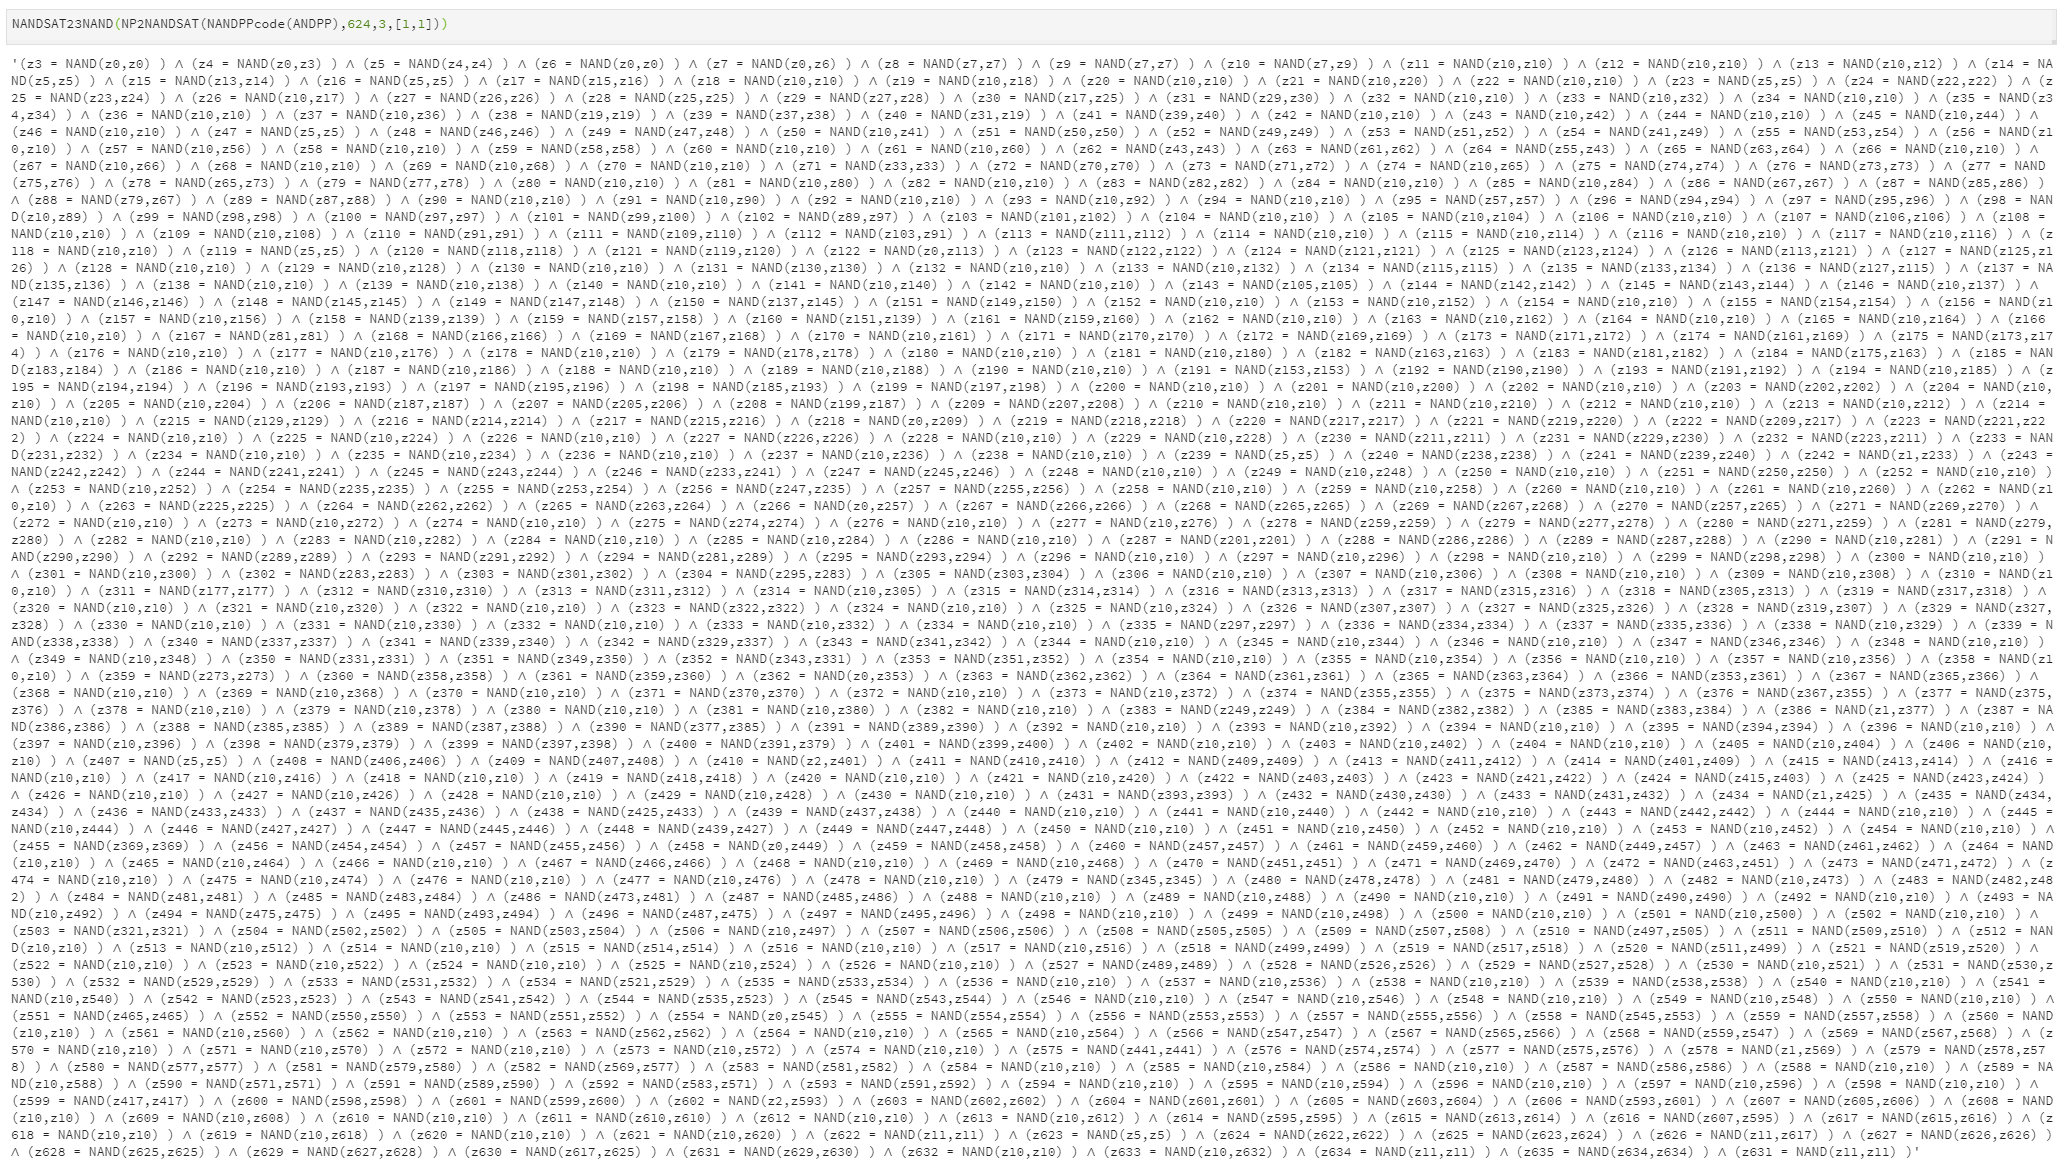
\includegraphics[width=\linewidth, height=1.5in, keepaspectratio]{../figure/threenandresultreduction.png}
\caption{A \(3\ensuremath{\mathit{NAND}}\) instance that is obtained by
taking a NAND-TM program for computing the \(\ensuremath{\mathit{AND}}\)
function, unrolling it to obtain a \(\ensuremath{\mathit{NANDSAT}}\)
instance, and then composing it with the reduction of
\cref{threenand-thm}.}
\label{resultreduction}
\end{marginfigure}

\section{From \(3\ensuremath{\mathit{NAND}}\) to
\(3\ensuremath{\mathit{SAT}}\)}\label{From-ensuremathmathitNAND}

The final step in the proof of \cref{cook-levin-thm} is the following:

\hypertarget{threenand-sat-thm}{}
\begin{lemma} \label[lemma]{threenand-sat-thm}

\(3\ensuremath{\mathit{NAND}} \leq_p 3\ensuremath{\mathit{SAT}}\).

\end{lemma}

\begin{proofidea} \label[proofidea]{To-prove-crefthreenand-sa}

To prove \cref{threenand-sat-thm} we need to map a 3NAND formula
\(\varphi\) into a 3SAT formula \(\psi\) such that \(\varphi\) is
satisfiable if and only if \(\psi\) is. The idea is that we can
transform every NAND constraint of the form
\(a=\ensuremath{\mathit{NAND}}(b,c)\) into the AND of ORs involving the
variables \(a,b,c\) and their negations, where each of the ORs contains
at most three terms. The construction is fairly straightforward, and the
details are given below.

\end{proofidea}

\begin{pause} \label[pause]{It-is-a-good-exercise-for}

It is a good exercise for you to try to find a 3CNF formula \(\xi\) on
three variables \(a,b,c\) such that \(\xi(a,b,c)\) is true if and only
if \(a = \ensuremath{\mathit{NAND}}(b,c)\). Once you do so, try to see
why this implies a reduction from \(3\ensuremath{\mathit{NAND}}\) to
\(3\ensuremath{\mathit{SAT}}\), and hence completes the proof of
\cref{threenand-sat-thm}

\end{pause}


\begin{figure}
\centering
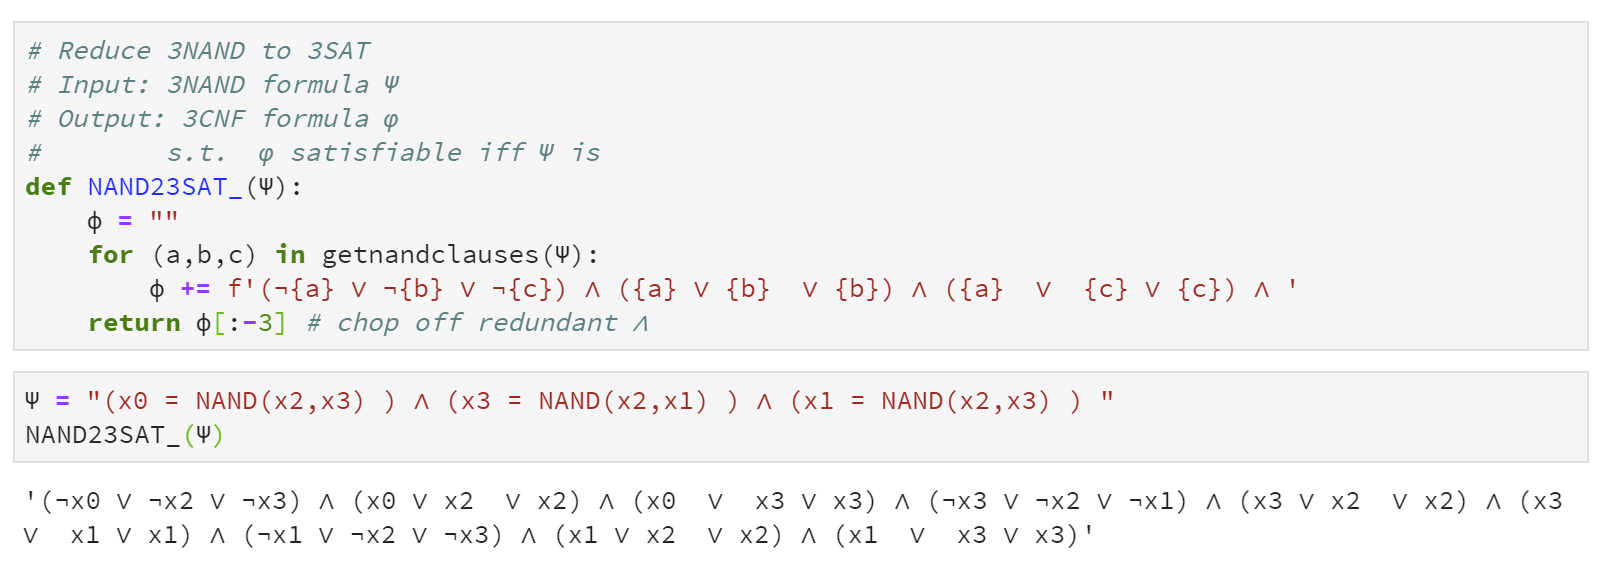
\includegraphics[width=\textwidth, height=0.25\paperheight, keepaspectratio]{../figure/3nandto3sat.png}
\caption{Code and example output for the reduction given in
\cref{threenand-sat-thm} of \(3\ensuremath{\mathit{NAND}}\) to
\(3\ensuremath{\mathit{SAT}}\).}
\label{threenandtothreesat}
\end{figure}

\begin{proof}[Proof of \cref{threenand-sat-thm}] \label[proof]{The-constraint-zi--ensure}

The constraint \[
z_i = \ensuremath{\mathit{NAND}}(z_j,z_k) \label{eq:NANDconstraint}
\] is satisfied if \(z_i=1\) whenever \((z_j,z_k) \neq (1,1)\). By going
through all cases, we can verify that \eqref{eq:NANDconstraint} is
equivalent to the constraint

\[
 (\overline{z_i} \vee \overline{z_j} \vee\overline{z_k} ) \wedge          (z_i     \vee z_j )
         \wedge  (z_i     \vee z_k) \;\;. \label{eq:CNFNAND}
\]

Indeed if \(z_j=z_k=1\) then the first constraint of \cref{eq:CNFNAND}
is only true if \(z_i=0\). On the other hand, if either of \(z_j\) or
\(z_k\) equals \(0\) then unless \(z_i=1\) either the second or third
constraints will fail. This means that, given any 3NAND formula
\(\varphi\) over \(n\) variables \(z_0,\ldots,z_{n-1}\), we can obtain a
3SAT formula \(\psi\) over the same variables by replacing every
\(3\ensuremath{\mathit{NAND}}\) constraint of \(\varphi\) with three
\(3\ensuremath{\mathit{OR}}\) constraints as in
\cref{eq:CNFNAND}.\footnote{The resulting formula will have some of the
  OR's involving only two variables. If we wanted to insist on each
  formula involving three distinct variables we can always add a ``dummy
  variable'' \(z_{n+m}\) and include it in all the OR's involving only
  two variables, and add a constraint requiring this dummy variable to
  be zero.} Because of the equivalence of \eqref{eq:NANDconstraint} and
\eqref{eq:CNFNAND}, the formula \(\psi\) satisfies that
\(\psi(z_0,\ldots,z_{n-1})=\varphi(z_0,\ldots,z_{n-1})\) for every
assignment \(z_0,\ldots,z_{n-1} \in \{0,1\}^n\) to the variables. In
particular \(\psi\) is satisfiable if and only if \(\varphi\) is, thus
completing the proof.

\end{proof}


\begin{figure}
\centering
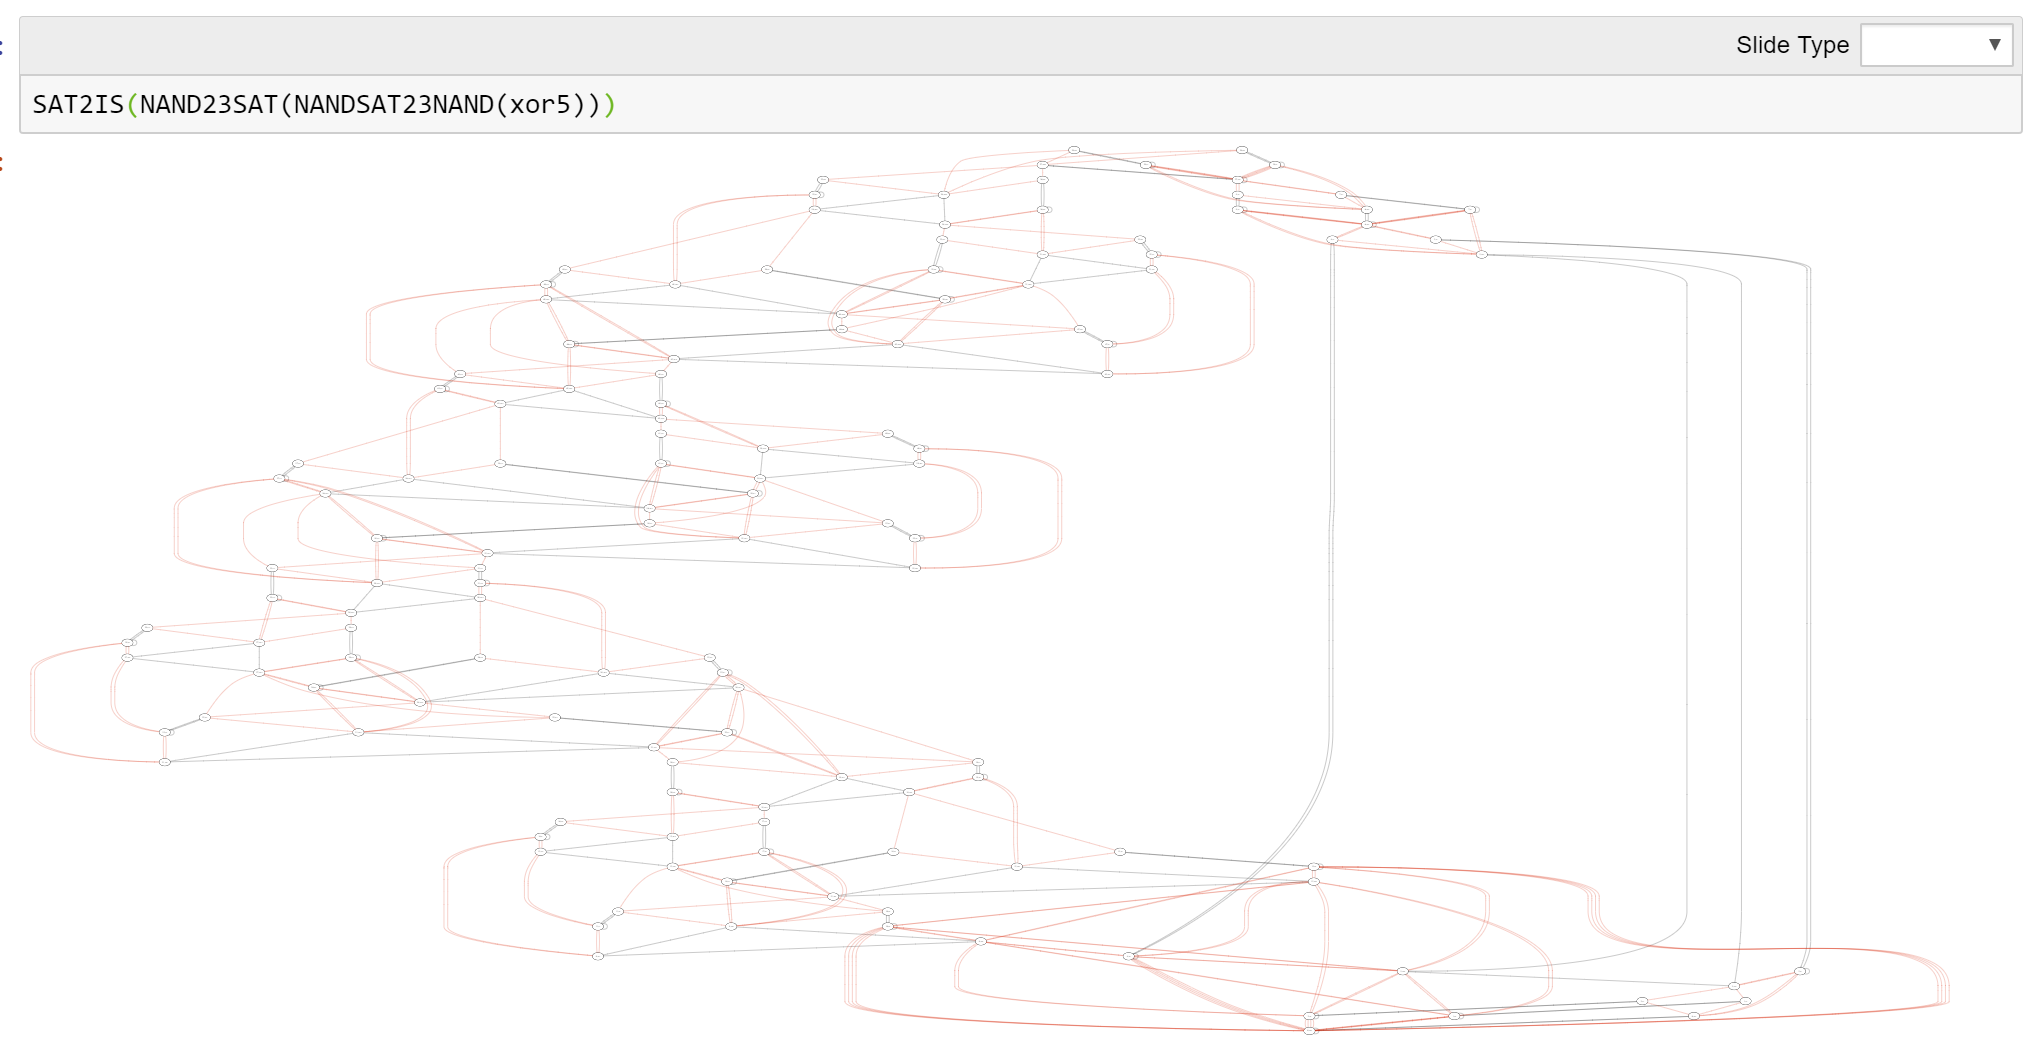
\includegraphics[width=\textwidth, height=0.25\paperheight, keepaspectratio]{../figure/indsetfromnandsat.png}
\caption{An instance of the \emph{independent set} problem obtained by
applying the reductions
\(\ensuremath{\mathit{NANDSAT}} \leq_p 3\ensuremath{\mathit{NAND}} \leq_p 3\ensuremath{\mathit{SAT}} \leq_p \ensuremath{\mathit{ISAT}}\)
starting with the \texttt{xor5} NAND-CIRC program.}
\label{indsetfromnandsatfig}
\end{figure}

\section{Wrapping up}\label{Wrapping-up}

We have shown that for every function \(F\) in \(\mathbf{NP}\),
\(F \leq_p \ensuremath{\mathit{NANDSAT}} \leq_p 3\ensuremath{\mathit{NAND}} \leq_p 3\ensuremath{\mathit{SAT}}\),
and so \(3\ensuremath{\mathit{SAT}}\) is \(\mathbf{NP}\)-hard. Since in
\cref{reductionchap} we saw that
\(3\ensuremath{\mathit{SAT}} \leq_p \ensuremath{\mathit{QUADEQ}}\),
\(3\ensuremath{\mathit{SAT}} \leq_p \ensuremath{\mathit{ISET}}\),
\(3\ensuremath{\mathit{SAT}} \leq_p \ensuremath{\mathit{MAXCUT}}\) and
\(3\ensuremath{\mathit{SAT}} \leq_p \ensuremath{\mathit{LONGPATH}}\),
all these problems are \(\mathbf{NP}\)-hard as well. Finally, since all
the aforementioned problems are in \(\mathbf{NP}\), they are all in fact
\(\mathbf{NP}\)-complete and have equivalent complexity. There are
thousands of other natural problems that are \(\mathbf{NP}\)-complete as
well. Finding a polynomial-time algorithm for any one of them will imply
a polynomial-time algorithm for all of them.


\begin{figure}
\centering
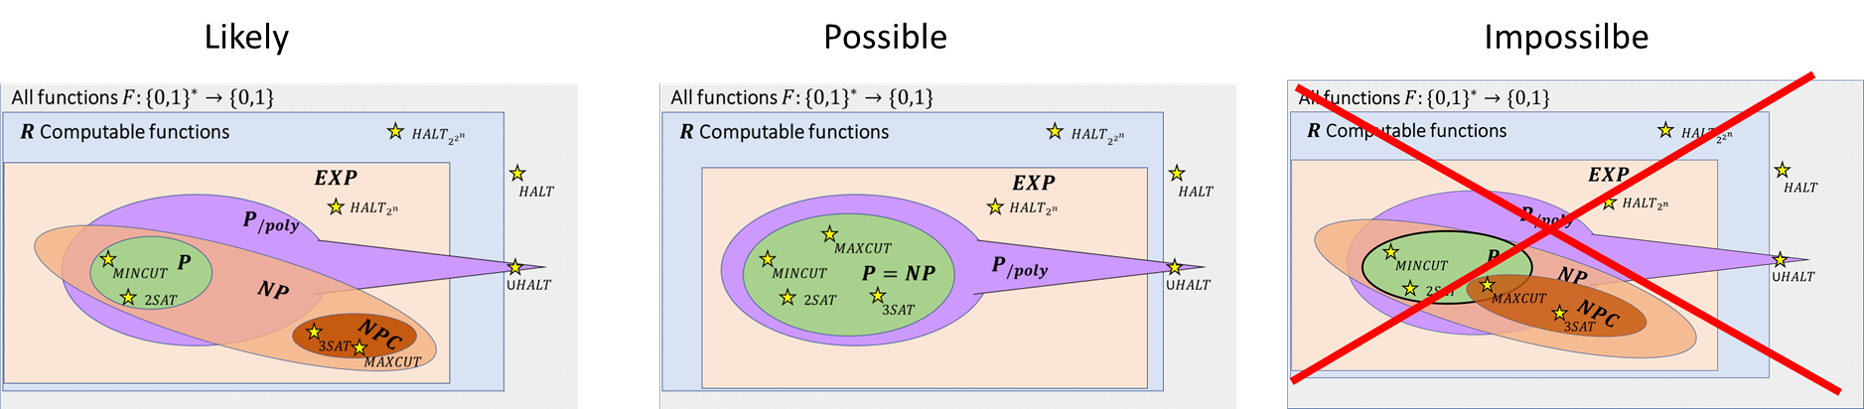
\includegraphics[width=\textwidth, height=0.25\paperheight, keepaspectratio]{../figure/inclusion_npc.png}
\caption{We believe that \(\mathbf{P} \neq \mathbf{NP}\) and all
\(\mathbf{NP}\) complete problems lie outside of \(\mathbf{P}\), but we
cannot rule out the possiblity that \(\mathbf{P}=\mathbf{NP}\). However,
we can rule out the possiblity that \emph{some} \(\mathbf{NP}\)-complete
problems are in \(\mathbf{P}\) and other do not, since we know that if
even one \(\mathbf{NP}\)-complete problem is in \(\mathbf{P}\) then
\(\mathbf{P}=\mathbf{NP}\). The relation between \(\mathbf{P_{/poly}}\)
and \(\mathbf{NP}\) is not known though it can be shown that if one
\(\mathbf{NP}\)-complete problem is in \(\mathbf{P_{/poly}}\) then
\(\mathbf{NP} \subseteq \mathbf{P_{/poly}}\).}
\label{npcinclusionfig}
\end{figure}

\begin{recap} \label[recap]{Many-of-the-problems-for-}

\begin{itemize}
\tightlist
\item
  Many of the problems for which we don't know polynomial-time
  algorithms are \(\mathbf{NP}\)-complete, which means that finding a
  polynomial-time algorithm for one of them would imply a
  polynomial-time algorithm for \emph{all} of them.
\item
  It is conjectured that \(\mathbf{NP}\neq \mathbf{P}\) which means that
  we believe that polynomial-time algorithms for these problems are not
  merely \emph{unknown} but are \emph{nonexistent}.
\item
  While an \(\mathbf{NP}\)-hardness result means for example that a
  full-fledged ``textbook'' solution to a problem such as MAX-CUT that
  is as clean and general as the algorithm for MIN-CUT probably does not
  exist, it does not mean that we need to give up whenever we see a
  MAX-CUT instance. Later in this course we will discuss several
  strategies to deal with \(\mathbf{NP}\)-hardness, including
  \emph{average-case complexity} and \emph{approximation algorithms}.
\end{itemize}

\end{recap}

\section{Exercises}\label{Exercises}

\hypertarget{ladner-ex}{}
\begin{exercise}[Poor man's Ladner's Theorem] \label[exercise]{ladner-ex}

Prove that if there is no \(n^{O(\log^2 n)}\) time algorithm for
\(3\ensuremath{\mathit{SAT}}\) then there is some \(F\in \mathbf{NP}\)
such that \(F \not\in \mathbf{P}\) and \(F\) is not \(\mathbf{NP}\)
complete.\footnote{\textbf{Hint:} Use the function \(F\) that on input a
  formula \(\varphi\) and a string of the form \(1^t\), outputs \(1\) if
  and only if \(\varphi\) is satisfiable and
  \(t=|\varphi|^{\log|\varphi|}\).}

\end{exercise}

\hypertarget{npconppnpex}{}
\begin{exercise}[$\mathbf{NP} \neq \mathbf{co-NP} \Rightarrow \mathbf{NP} \neq \mathbf{P}$] \label[exercise]{npconppnpex}

Let \(\overline{3\ensuremath{\mathit{SAT}}}\) be the function that on
input a 3CNF formula \(\varphi\) return
\(1-3\ensuremath{\mathit{SAT}}(\varphi)\). Prove that if
\(\overline{3\ensuremath{\mathit{SAT}}} \not\in \mathbf{NP}\) then
\(\mathbf{P} \neq \mathbf{NP}\). See footnote for hint.\footnote{\emph{Hint:}
  Prove and then use the fact that \(\mathbf{P}\) \emph{is} closed under
  complement.}

\end{exercise}

\hypertarget{WSATex}{}
\begin{exercise} \label[exercise]{WSATex}

Define \(\ensuremath{\mathit{WSAT}}\) to be the following function: the
input is a CNF formula \(\varphi\) where each clause is the OR of one to
three variables (\emph{without negations}), and a number
\(k\in \mathbb{N}\). For example, the following formula can be used for
a valid input to \(\ensuremath{\mathit{WSAT}}\):
\(\varphi = (x_5 \vee x_{2} \vee x_1) \wedge (x_1 \vee x_3 \vee x_0) \wedge (x_2 \vee x_4 \vee x_0)\).
The output \(\ensuremath{\mathit{WSAT}}(\varphi,k)=1\) if and only if
there exists a satisfying assignment to \(\varphi\) in which exactly
\(k\) of the variables get the value \(1\). For example for the formula
above \(\ensuremath{\mathit{WSAT}}(\varphi,2)=1\) since the assignment
\((1,1,0,0,0,0)\) satisfies all the clauses. However
\(\ensuremath{\mathit{WSAT}}(\varphi,1)=0\) since there is no single
variable appearing in all clauses.

Prove that \(\ensuremath{\mathit{WSAT}}\) is \(\mathbf{NP}\)-complete.

\end{exercise}

\hypertarget{employeerecrutingex}{}
\begin{exercise} \label[exercise]{employeerecrutingex}

In the \emph{employee recruiting problem} we are given a list of
potential employees, each of which has some subset of \(m\) potential
skills, and a number \(k\). We need to assemble a team of \(k\)
employees such that for every skill there would be one member of the
team with this skill.

For example, if Alice has the skills ``C programming'', ``NAND
programming'' and ``Solving Differential Equations'', Bob has the skills
``C programming'' and ``Solving Differential Equations'', and Charlie
has the skills ``NAND programming'' and ``Coffee Brewing'', then if we
want a team of two people that covers all the four skills, we would hire
Alice and Charlie.

Define the function \(\ensuremath{\mathit{EMP}}\) s.t. on input the
skills \(L\) of all potential employees (in the form of a sequence \(L\)
of \(n\) lists \(L_1,\ldots,L_n\), each containing distinct numbers
between \(0\) and \(m\)), and a number \(k\),
\(\ensuremath{\mathit{EMP}}(L,k)=1\) if and only if there is a subset
\(S\) of \(k\) potential employees such that for every skill \(j\) in
\([m]\), there is an employee in \(S\) that has the skill \(j\).

Prove that \(\ensuremath{\mathit{EMP}}\) is \(\mathbf{NP}\) complete.

\end{exercise}

\hypertarget{balancedmc}{}
\begin{exercise}[Balanced max cut] \label[exercise]{balancedmc}

Prove that the ``balanced variant'' of the maximum cut problem is
\(\mathbf{NP}\)-complete, where this is defined as
\(\ensuremath{\mathit{BMC}}:\{0,1\}^* \rightarrow \{0,1\}\) where for
every graph \(G=(V,E)\) and \(k\in \mathbb{N}\),
\(\ensuremath{\mathit{BMC}}(G,k)=1\) if and only if there exists a cut
\(S\) in \(G\) cutting at least \(k\) edges such that \(|S|=|V|/2\).

\end{exercise}

\hypertarget{manyregs}{}
\begin{exercise}[Regular expression intersection] \label[exercise]{manyregs}

Let \(\ensuremath{\mathit{MANYREGS}}\) be the following function: On
input a list of regular expressions \(exp_0,\ldots,\exp_m\) (represented
as strings in some standard way), output \(1\) if and only if there is a
single string \(x \in \{0,1\}^*\) that matches all of them. Prove that
\(\ensuremath{\mathit{MANYREGS}}\) is \(\mathbf{NP}\)-hard.

\end{exercise}

\section{Bibliographical notes}\label{Bibliographical-notes}

Aaronson's 120 page survey \cite{aaronson2016p} is a beautiful and
extensive exposition to the \(\mathbf{P}\) vs \(\mathbf{NP}\) problem,
its importance and status. See also as well as Chapter 3 in Wigderson's
excellent book \cite{wigderson2017mathematics}. Johnson
\cite{johnson2012brief} gives a survey of the historical development of
the theory of \(\mathbf{NP}\) completeness. The following
\href{https://goo.gl/bFHsd9}{web page} keeps a catalog of failed
attempts at settling \(\mathbf{P}\) vs \(\mathbf{NP}\). At the time of
this writing, it lists about 110 papers claiming to resolve the
question, of which about 60 claim to prove that
\(\mathbf{P}=\mathbf{NP}\) and about 50 claim to prove that
\(\mathbf{P} \neq \mathbf{NP}\).

Eugene Lawler's quote on the ``mystical power of twoness'' was taken
from the wonderful book ``The Nature of Computation'' by Moore and
Mertens. See also
\href{https://pure.tue.nl/ws/files/1506049/511307.pdf}{this memorial
essay on Lawler} by Lenstra.
